\documentclass[12pt]{article}
\usepackage[margin=0.1in]{geometry}
\usepackage{xcolor}
\usepackage{framed}
\usepackage{enumitem}
\usepackage{adjustbox}
\usepackage{natbib}
\usepackage{chngpage}
\usepackage{mathtools,xparse}
\usepackage{graphics}
\usepackage{tikz}
\usepackage{tabu}
\usepackage{tikz-cd}
\colorlet{shadecolor}{orange!15}
% \definecolor{shadecolor}{rgb}{255,128,0}\
\usepackage{float}
\usepackage{fullpage} % Package to use full page
\usepackage{parskip} % Package to tweak paragraph skipping
\usepackage{amsmath}
\usepackage{amssymb}
\usepackage{hyperref}
\usepackage{pdflscape}
\usepackage{setspace}
\usepackage{graphicx} % Allows including images
\usepackage{booktabs} % Allows the use of \toprule, \midrule and \bottomrule in tables
\usepackage{longtable}
\usepackage{indentfirst}
\usetikzlibrary{arrows,shapes,positioning,shadows,trees}
\usepackage{array}
\usepackage{wrapfig}
\usepackage{multirow}
\usepackage{pdflscape}
\usepackage{threeparttable}
\usepackage{makecell}
\usepackage[normalem]{ulem}
\newcommand{\PreserveBackslash}[1]{\let\temp=\\#1\let\\=\temp}
\newcolumntype{L}[1]{>{\PreserveBackslash\raggedright}m{#1}}
\newcolumntype{R}[1]{>{\PreserveBackslash}p{#1}}
\newcolumntype{C}[1]{>{\PreserveBackslash\centering}m{#1}}

\newcommand{\mc}[3]{\multicolumn{#1}{#2}{#3}}

\tikzset{
  basic/.style  = {draw, text width=2cm, drop shadow, font=\sffamily, rectangle},
  root/.style   = {basic, rounded corners=2pt, thin, align=center,
                   fill=green!30},
  level 2/.style = {basic, rounded corners=6pt, thin,align=center, fill=green!60,
                   text width=8em},
  level 3/.style = {basic, thin, align=left, fill=pink!60, text width=6.5em}
}


\newcommand\independent{\protect\mathpalette{\protect\independenT}{\perp}}
\newcommand\gamij{\mathbf{\gamma_{ij}}}
\def\independenT#1#2{\mathrel{\rlap{$#1#2$}\mkern2mu{#1#2}}}
\newcommand\params{(p_M, p_{M\ell}, p_{U\ell})}
\newcommand\longparam{(L,n_1,n_2, p_M,p_{M\ell},p_{U\ell})}


%Allows multi-column tables 
% Macros for Scientific Word and Scientific WorkPlace 5.5 documents saved with the LaTeX filter.
% Copyright (C) 2005 Mackichan Software, Inc.

\typeout{TCILATEX Macros for Scientific Word and Scientific WorkPlace 5.5 <06 Oct 2005>.}
\typeout{NOTICE:  This macro file is NOT proprietary and may be 
freely copied and distributed.}
%
\makeatletter

%%%%%%%%%%%%%%%%%%%%%
% pdfTeX related.
\ifx\pdfoutput\relax\let\pdfoutput=\undefined\fi
\newcount\msipdfoutput
\ifx\pdfoutput\undefined
\else
 \ifcase\pdfoutput
 \else 
    \msipdfoutput=1
    \ifx\paperwidth\undefined
    \else
      \ifdim\paperheight=0pt\relax
      \else
        \pdfpageheight\paperheight
      \fi
      \ifdim\paperwidth=0pt\relax
      \else
        \pdfpagewidth\paperwidth
      \fi
    \fi
  \fi  
\fi

%%%%%%%%%%%%%%%%%%%%%
% FMTeXButton
% This is used for putting TeXButtons in the 
% frontmatter of a document. Add a line like
% \QTagDef{FMTeXButton}{101}{} to the filter 
% section of the cst being used. Also add a
% new section containing:
%     [f_101]
%     ALIAS=FMTexButton
%     TAG_TYPE=FIELD
%     TAG_LEADIN=TeX Button:
%
% It also works to put \defs in the preamble after 
% the \input tcilatex
\def\FMTeXButton#1{#1}
%
%%%%%%%%%%%%%%%%%%%%%%
% macros for time
\newcount\@hour\newcount\@minute\chardef\@x10\chardef\@xv60
\def\tcitime{
\def\@time{%
  \@minute\time\@hour\@minute\divide\@hour\@xv
  \ifnum\@hour<\@x 0\fi\the\@hour:%
  \multiply\@hour\@xv\advance\@minute-\@hour
  \ifnum\@minute<\@x 0\fi\the\@minute
  }}%

%%%%%%%%%%%%%%%%%%%%%%
% macro for hyperref and msihyperref
%\@ifundefined{hyperref}{\def\hyperref#1#2#3#4{#2\ref{#4}#3}}{}

\def\x@hyperref#1#2#3{%
   % Turn off various catcodes before reading parameter 4
   \catcode`\~ = 12
   \catcode`\$ = 12
   \catcode`\_ = 12
   \catcode`\# = 12
   \catcode`\& = 12
   \catcode`\% = 12
   \y@hyperref{#1}{#2}{#3}%
}

\def\y@hyperref#1#2#3#4{%
   #2\ref{#4}#3
   \catcode`\~ = 13
   \catcode`\$ = 3
   \catcode`\_ = 8
   \catcode`\# = 6
   \catcode`\& = 4
   \catcode`\% = 14
}

\@ifundefined{hyperref}{\let\hyperref\x@hyperref}{}
\@ifundefined{msihyperref}{\let\msihyperref\x@hyperref}{}




% macro for external program call
\@ifundefined{qExtProgCall}{\def\qExtProgCall#1#2#3#4#5#6{\relax}}{}
%%%%%%%%%%%%%%%%%%%%%%
%
% macros for graphics
%
\def\FILENAME#1{#1}%
%
\def\QCTOpt[#1]#2{%
  \def\QCTOptB{#1}
  \def\QCTOptA{#2}
}
\def\QCTNOpt#1{%
  \def\QCTOptA{#1}
  \let\QCTOptB\empty
}
\def\Qct{%
  \@ifnextchar[{%
    \QCTOpt}{\QCTNOpt}
}
\def\QCBOpt[#1]#2{%
  \def\QCBOptB{#1}%
  \def\QCBOptA{#2}%
}
\def\QCBNOpt#1{%
  \def\QCBOptA{#1}%
  \let\QCBOptB\empty
}
\def\Qcb{%
  \@ifnextchar[{%
    \QCBOpt}{\QCBNOpt}%
}
\def\PrepCapArgs{%
  \ifx\QCBOptA\empty
    \ifx\QCTOptA\empty
      {}%
    \else
      \ifx\QCTOptB\empty
        {\QCTOptA}%
      \else
        [\QCTOptB]{\QCTOptA}%
      \fi
    \fi
  \else
    \ifx\QCBOptA\empty
      {}%
    \else
      \ifx\QCBOptB\empty
        {\QCBOptA}%
      \else
        [\QCBOptB]{\QCBOptA}%
      \fi
    \fi
  \fi
}
\newcount\GRAPHICSTYPE
%\GRAPHICSTYPE 0 is for TurboTeX
%\GRAPHICSTYPE 1 is for DVIWindo (PostScript)
%%%(removed)%\GRAPHICSTYPE 2 is for psfig (PostScript)
\GRAPHICSTYPE=\z@
\def\GRAPHICSPS#1{%
 \ifcase\GRAPHICSTYPE%\GRAPHICSTYPE=0
   \special{ps: #1}%
 \or%\GRAPHICSTYPE=1
   \special{language "PS", include "#1"}%
%%%\or%\GRAPHICSTYPE=2
%%%  #1%
 \fi
}%
%
\def\GRAPHICSHP#1{\special{include #1}}%
%
% \graffile{ body }                                  %#1
%          { contentswidth (scalar)  }               %#2
%          { contentsheight (scalar) }               %#3
%          { vertical shift when in-line (scalar) }  %#4

\def\graffile#1#2#3#4{%
%%% \ifnum\GRAPHICSTYPE=\tw@
%%%  %Following if using psfig
%%%  \@ifundefined{psfig}{\input psfig.tex}{}%
%%%  \psfig{file=#1, height=#3, width=#2}%
%%% \else
  %Following for all others
  % JCS - added BOXTHEFRAME, see below
    \bgroup
	   \@inlabelfalse
       \leavevmode
       \@ifundefined{bbl@deactivate}{\def~{\string~}}{\activesoff}%
        \raise -#4 \BOXTHEFRAME{%
           \hbox to #2{\raise #3\hbox to #2{\null #1\hfil}}}%
    \egroup
}%
%
% A box for drafts
\def\draftbox#1#2#3#4{%
 \leavevmode\raise -#4 \hbox{%
  \frame{\rlap{\protect\tiny #1}\hbox to #2%
   {\vrule height#3 width\z@ depth\z@\hfil}%
  }%
 }%
}%
%
\newcount\@msidraft
\@msidraft=\z@
\let\nographics=\@msidraft
\newif\ifwasdraft
\wasdraftfalse

%  \GRAPHIC{ body }                                  %#1
%          { draft name }                            %#2
%          { contentswidth (scalar)  }               %#3
%          { contentsheight (scalar) }               %#4
%          { vertical shift when in-line (scalar) }  %#5
\def\GRAPHIC#1#2#3#4#5{%
   \ifnum\@msidraft=\@ne\draftbox{#2}{#3}{#4}{#5}%
   \else\graffile{#1}{#3}{#4}{#5}%
   \fi
}
%
\def\addtoLaTeXparams#1{%
    \edef\LaTeXparams{\LaTeXparams #1}}%
%
% JCS -  added a switch BoxFrame that can 
% be set by including X in the frame params.
% If set a box is drawn around the frame.

\newif\ifBoxFrame \BoxFramefalse
\newif\ifOverFrame \OverFramefalse
\newif\ifUnderFrame \UnderFramefalse

\def\BOXTHEFRAME#1{%
   \hbox{%
      \ifBoxFrame
         \frame{#1}%
      \else
         {#1}%
      \fi
   }%
}


\def\doFRAMEparams#1{\BoxFramefalse\OverFramefalse\UnderFramefalse\readFRAMEparams#1\end}%
\def\readFRAMEparams#1{%
 \ifx#1\end%
  \let\next=\relax
  \else
  \ifx#1i\dispkind=\z@\fi
  \ifx#1d\dispkind=\@ne\fi
  \ifx#1f\dispkind=\tw@\fi
  \ifx#1t\addtoLaTeXparams{t}\fi
  \ifx#1b\addtoLaTeXparams{b}\fi
  \ifx#1p\addtoLaTeXparams{p}\fi
  \ifx#1h\addtoLaTeXparams{h}\fi
  \ifx#1X\BoxFrametrue\fi
  \ifx#1O\OverFrametrue\fi
  \ifx#1U\UnderFrametrue\fi
  \ifx#1w
    \ifnum\@msidraft=1\wasdrafttrue\else\wasdraftfalse\fi
    \@msidraft=\@ne
  \fi
  \let\next=\readFRAMEparams
  \fi
 \next
 }%
%
%Macro for In-line graphics object
%   \IFRAME{ contentswidth (scalar)  }               %#1
%          { contentsheight (scalar) }               %#2
%          { vertical shift when in-line (scalar) }  %#3
%          { draft name }                            %#4
%          { body }                                  %#5
%          { caption}                                %#6


\def\IFRAME#1#2#3#4#5#6{%
      \bgroup
      \let\QCTOptA\empty
      \let\QCTOptB\empty
      \let\QCBOptA\empty
      \let\QCBOptB\empty
      #6%
      \parindent=0pt
      \leftskip=0pt
      \rightskip=0pt
      \setbox0=\hbox{\QCBOptA}%
      \@tempdima=#1\relax
      \ifOverFrame
          % Do this later
          \typeout{This is not implemented yet}%
          \show\HELP
      \else
         \ifdim\wd0>\@tempdima
            \advance\@tempdima by \@tempdima
            \ifdim\wd0 >\@tempdima
               \setbox1 =\vbox{%
                  \unskip\hbox to \@tempdima{\hfill\GRAPHIC{#5}{#4}{#1}{#2}{#3}\hfill}%
                  \unskip\hbox to \@tempdima{\parbox[b]{\@tempdima}{\QCBOptA}}%
               }%
               \wd1=\@tempdima
            \else
               \textwidth=\wd0
               \setbox1 =\vbox{%
                 \noindent\hbox to \wd0{\hfill\GRAPHIC{#5}{#4}{#1}{#2}{#3}\hfill}\\%
                 \noindent\hbox{\QCBOptA}%
               }%
               \wd1=\wd0
            \fi
         \else
            \ifdim\wd0>0pt
              \hsize=\@tempdima
              \setbox1=\vbox{%
                \unskip\GRAPHIC{#5}{#4}{#1}{#2}{0pt}%
                \break
                \unskip\hbox to \@tempdima{\hfill \QCBOptA\hfill}%
              }%
              \wd1=\@tempdima
           \else
              \hsize=\@tempdima
              \setbox1=\vbox{%
                \unskip\GRAPHIC{#5}{#4}{#1}{#2}{0pt}%
              }%
              \wd1=\@tempdima
           \fi
         \fi
         \@tempdimb=\ht1
         %\advance\@tempdimb by \dp1
         \advance\@tempdimb by -#2
         \advance\@tempdimb by #3
         \leavevmode
         \raise -\@tempdimb \hbox{\box1}%
      \fi
      \egroup%
}%
%
%Macro for Display graphics object
%   \DFRAME{ contentswidth (scalar)  }               %#1
%          { contentsheight (scalar) }               %#2
%          { draft label }                           %#3
%          { name }                                  %#4
%          { caption}                                %#5
\def\DFRAME#1#2#3#4#5{%
  \vspace\topsep
  \hfil\break
  \bgroup
     \leftskip\@flushglue
	 \rightskip\@flushglue
	 \parindent\z@
	 \parfillskip\z@skip
     \let\QCTOptA\empty
     \let\QCTOptB\empty
     \let\QCBOptA\empty
     \let\QCBOptB\empty
	 \vbox\bgroup
        \ifOverFrame 
           #5\QCTOptA\par
        \fi
        \GRAPHIC{#4}{#3}{#1}{#2}{\z@}%
        \ifUnderFrame 
           \break#5\QCBOptA
        \fi
	 \egroup
  \egroup
  \vspace\topsep
  \break
}%
%
%Macro for Floating graphic object
%   \FFRAME{ framedata f|i tbph x F|T }              %#1
%          { contentswidth (scalar)  }               %#2
%          { contentsheight (scalar) }               %#3
%          { caption }                               %#4
%          { label }                                 %#5
%          { draft name }                            %#6
%          { body }                                  %#7
\def\FFRAME#1#2#3#4#5#6#7{%
 %If float.sty loaded and float option is 'h', change to 'H'  (gp) 1998/09/05
  \@ifundefined{floatstyle}
    {%floatstyle undefined (and float.sty not present), no change
     \begin{figure}[#1]%
    }
    {%floatstyle DEFINED
	 \ifx#1h%Only the h parameter, change to H
      \begin{figure}[H]%
	 \else
      \begin{figure}[#1]%
	 \fi
	}
  \let\QCTOptA\empty
  \let\QCTOptB\empty
  \let\QCBOptA\empty
  \let\QCBOptB\empty
  \ifOverFrame
    #4
    \ifx\QCTOptA\empty
    \else
      \ifx\QCTOptB\empty
        \caption{\QCTOptA}%
      \else
        \caption[\QCTOptB]{\QCTOptA}%
      \fi
    \fi
    \ifUnderFrame\else
      \label{#5}%
    \fi
  \else
    \UnderFrametrue%
  \fi
  \begin{center}\GRAPHIC{#7}{#6}{#2}{#3}{\z@}\end{center}%
  \ifUnderFrame
    #4
    \ifx\QCBOptA\empty
      \caption{}%
    \else
      \ifx\QCBOptB\empty
        \caption{\QCBOptA}%
      \else
        \caption[\QCBOptB]{\QCBOptA}%
      \fi
    \fi
    \label{#5}%
  \fi
  \end{figure}%
 }%
%
%
%    \FRAME{ framedata f|i tbph x F|T }              %#1
%          { contentswidth (scalar)  }               %#2
%          { contentsheight (scalar) }               %#3
%          { vertical shift when in-line (scalar) }  %#4
%          { caption }                               %#5
%          { label }                                 %#6
%          { name }                                  %#7
%          { body }                                  %#8
%
%    framedata is a string which can contain the following
%    characters: idftbphxFT
%    Their meaning is as follows:
%             i, d or f : in-line, display, or floating
%             t,b,p,h   : LaTeX floating placement options
%             x         : fit contents box to contents
%             F or T    : Figure or Table. 
%                         Later this can expand
%                         to a more general float class.
%
%
\newcount\dispkind%

\def\makeactives{
  \catcode`\"=\active
  \catcode`\;=\active
  \catcode`\:=\active
  \catcode`\'=\active
  \catcode`\~=\active
}
\bgroup
   \makeactives
   \gdef\activesoff{%
      \def"{\string"}%
      \def;{\string;}%
      \def:{\string:}%
      \def'{\string'}%
      \def~{\string~}%
      %\bbl@deactivate{"}%
      %\bbl@deactivate{;}%
      %\bbl@deactivate{:}%
      %\bbl@deactivate{'}%
    }
\egroup

\def\FRAME#1#2#3#4#5#6#7#8{%
 \bgroup
 \ifnum\@msidraft=\@ne
   \wasdrafttrue
 \else
   \wasdraftfalse%
 \fi
 \def\LaTeXparams{}%
 \dispkind=\z@
 \def\LaTeXparams{}%
 \doFRAMEparams{#1}%
 \ifnum\dispkind=\z@\IFRAME{#2}{#3}{#4}{#7}{#8}{#5}\else
  \ifnum\dispkind=\@ne\DFRAME{#2}{#3}{#7}{#8}{#5}\else
   \ifnum\dispkind=\tw@
    \edef\@tempa{\noexpand\FFRAME{\LaTeXparams}}%
    \@tempa{#2}{#3}{#5}{#6}{#7}{#8}%
    \fi
   \fi
  \fi
  \ifwasdraft\@msidraft=1\else\@msidraft=0\fi{}%
  \egroup
 }%
%
% This macro added to let SW gobble a parameter that
% should not be passed on and expanded. 

\def\TEXUX#1{"texux"}

%
% Macros for text attributes:
%
\def\BF#1{{\bf {#1}}}%
\def\NEG#1{\leavevmode\hbox{\rlap{\thinspace/}{$#1$}}}%
%
%%%%%%%%%%%%%%%%%%%%%%%%%%%%%%%%%%%%%%%%%%%%%%%%%%%%%%%%%%%%%%%%%%%%%%%%
%
%
% macros for user - defined functions
\def\limfunc#1{\mathop{\rm #1}}%
\def\func#1{\mathop{\rm #1}\nolimits}%
% macro for unit names
\def\unit#1{\mathord{\thinspace\rm #1}}%

%
% miscellaneous 
\long\def\QQQ#1#2{%
     \long\expandafter\def\csname#1\endcsname{#2}}%
\@ifundefined{QTP}{\def\QTP#1{}}{}
\@ifundefined{QEXCLUDE}{\def\QEXCLUDE#1{}}{}
\@ifundefined{Qlb}{\def\Qlb#1{#1}}{}
\@ifundefined{Qlt}{\def\Qlt#1{#1}}{}
\def\QWE{}%
\long\def\QQA#1#2{}%
\def\QTR#1#2{{\csname#1\endcsname {#2}}}%
  %	Add aliases for the ulem package
  \let\QQQuline\uline
  \let\QQQsout\sout
  \let\QQQuuline\uuline
  \let\QQQuwave\uwave
  \let\QQQxout\xout
\long\def\TeXButton#1#2{#2}%
\long\def\QSubDoc#1#2{#2}%
\def\EXPAND#1[#2]#3{}%
\def\NOEXPAND#1[#2]#3{}%
\def\PROTECTED{}%
\def\LaTeXparent#1{}%
\def\ChildStyles#1{}%
\def\ChildDefaults#1{}%
\def\QTagDef#1#2#3{}%

% Constructs added with Scientific Notebook
\@ifundefined{correctchoice}{\def\correctchoice{\relax}}{}
\@ifundefined{HTML}{\def\HTML#1{\relax}}{}
\@ifundefined{TCIIcon}{\def\TCIIcon#1#2#3#4{\relax}}{}
\if@compatibility
  \typeout{Not defining UNICODE  U or CustomNote commands for LaTeX 2.09.}
\else
  \providecommand{\UNICODE}[2][]{\protect\rule{.1in}{.1in}}
  \providecommand{\U}[1]{\protect\rule{.1in}{.1in}}
  \providecommand{\CustomNote}[3][]{\marginpar{#3}}
\fi

\@ifundefined{lambdabar}{
      \def\lambdabar{\errmessage{You have used the lambdabar symbol. 
                      This is available for typesetting only in RevTeX styles.}}
   }{}

%
% Macros for style editor docs
\@ifundefined{StyleEditBeginDoc}{\def\StyleEditBeginDoc{\relax}}{}
%
% Macros for footnotes
\def\QQfnmark#1{\footnotemark}
\def\QQfntext#1#2{\addtocounter{footnote}{#1}\footnotetext{#2}}
%
% Macros for indexing.
%
\@ifundefined{TCIMAKEINDEX}{}{\makeindex}%
%
% Attempts to avoid problems with other styles
\@ifundefined{abstract}{%
 \def\abstract{%
  \if@twocolumn
   \section*{Abstract (Not appropriate in this style!)}%
   \else \small 
   \begin{center}{\bf Abstract\vspace{-.5em}\vspace{\z@}}\end{center}%
   \quotation 
   \fi
  }%
 }{%
 }%
\@ifundefined{endabstract}{\def\endabstract
  {\if@twocolumn\else\endquotation\fi}}{}%
\@ifundefined{maketitle}{\def\maketitle#1{}}{}%
\@ifundefined{affiliation}{\def\affiliation#1{}}{}%
\@ifundefined{proof}{\def\proof{\noindent{\bfseries Proof. }}}{}%
\@ifundefined{endproof}{\def\endproof{\mbox{\ \rule{.1in}{.1in}}}}{}%
\@ifundefined{newfield}{\def\newfield#1#2{}}{}%
\@ifundefined{chapter}{\def\chapter#1{\par(Chapter head:)#1\par }%
 \newcount\c@chapter}{}%
\@ifundefined{part}{\def\part#1{\par(Part head:)#1\par }}{}%
\@ifundefined{section}{\def\section#1{\par(Section head:)#1\par }}{}%
\@ifundefined{subsection}{\def\subsection#1%
 {\par(Subsection head:)#1\par }}{}%
\@ifundefined{subsubsection}{\def\subsubsection#1%
 {\par(Subsubsection head:)#1\par }}{}%
\@ifundefined{paragraph}{\def\paragraph#1%
 {\par(Subsubsubsection head:)#1\par }}{}%
\@ifundefined{subparagraph}{\def\subparagraph#1%
 {\par(Subsubsubsubsection head:)#1\par }}{}%
%%%%%%%%%%%%%%%%%%%%%%%%%%%%%%%%%%%%%%%%%%%%%%%%%%%%%%%%%%%%%%%%%%%%%%%%
% These symbols are not recognized by LaTeX
\@ifundefined{therefore}{\def\therefore{}}{}%
\@ifundefined{backepsilon}{\def\backepsilon{}}{}%
\@ifundefined{yen}{\def\yen{\hbox{\rm\rlap=Y}}}{}%
\@ifundefined{registered}{%
   \def\registered{\relax\ifmmode{}\r@gistered
                    \else$\m@th\r@gistered$\fi}%
 \def\r@gistered{^{\ooalign
  {\hfil\raise.07ex\hbox{$\scriptstyle\rm\text{R}$}\hfil\crcr
  \mathhexbox20D}}}}{}%
\@ifundefined{Eth}{\def\Eth{}}{}%
\@ifundefined{eth}{\def\eth{}}{}%
\@ifundefined{Thorn}{\def\Thorn{}}{}%
\@ifundefined{thorn}{\def\thorn{}}{}%
% A macro to allow any symbol that requires math to appear in text
\def\TEXTsymbol#1{\mbox{$#1$}}%
\@ifundefined{degree}{\def\degree{{}^{\circ}}}{}%
%
% macros for T3TeX files
\newdimen\theight
\@ifundefined{Column}{\def\Column{%
 \vadjust{\setbox\z@=\hbox{\scriptsize\quad\quad tcol}%
  \theight=\ht\z@\advance\theight by \dp\z@\advance\theight by \lineskip
  \kern -\theight \vbox to \theight{%
   \rightline{\rlap{\box\z@}}%
   \vss
   }%
  }%
 }}{}%
%
\@ifundefined{qed}{\def\qed{%
 \ifhmode\unskip\nobreak\fi\ifmmode\ifinner\else\hskip5\p@\fi\fi
 \hbox{\hskip5\p@\vrule width4\p@ height6\p@ depth1.5\p@\hskip\p@}%
 }}{}%
%
\@ifundefined{cents}{\def\cents{\hbox{\rm\rlap c/}}}{}%
\@ifundefined{tciLaplace}{\def\tciLaplace{\ensuremath{\mathcal{L}}}}{}%
\@ifundefined{tciFourier}{\def\tciFourier{\ensuremath{\mathcal{F}}}}{}%
\@ifundefined{textcurrency}{\def\textcurrency{\hbox{\rm\rlap xo}}}{}%
\@ifundefined{texteuro}{\def\texteuro{\hbox{\rm\rlap C=}}}{}%
\@ifundefined{euro}{\def\euro{\hbox{\rm\rlap C=}}}{}%
\@ifundefined{textfranc}{\def\textfranc{\hbox{\rm\rlap-F}}}{}%
\@ifundefined{textlira}{\def\textlira{\hbox{\rm\rlap L=}}}{}%
\@ifundefined{textpeseta}{\def\textpeseta{\hbox{\rm P\negthinspace s}}}{}%
%
\@ifundefined{miss}{\def\miss{\hbox{\vrule height2\p@ width 2\p@ depth\z@}}}{}%
%
\@ifundefined{vvert}{\def\vvert{\Vert}}{}%  %always translated to \left| or \right|
%
\@ifundefined{tcol}{\def\tcol#1{{\baselineskip=6\p@ \vcenter{#1}} \Column}}{}%
%
\@ifundefined{dB}{\def\dB{\hbox{{}}}}{}%        %dummy entry in column 
\@ifundefined{mB}{\def\mB#1{\hbox{$#1$}}}{}%   %column entry
\@ifundefined{nB}{\def\nB#1{\hbox{#1}}}{}%     %column entry (not math)
%
\@ifundefined{note}{\def\note{$^{\dag}}}{}%
%
\def\newfmtname{LaTeX2e}
% No longer load latexsym.  This is now handled by SWP, which uses amsfonts if necessary
%
\ifx\fmtname\newfmtname
  \DeclareOldFontCommand{\rm}{\normalfont\rmfamily}{\mathrm}
  \DeclareOldFontCommand{\sf}{\normalfont\sffamily}{\mathsf}
  \DeclareOldFontCommand{\tt}{\normalfont\ttfamily}{\mathtt}
  \DeclareOldFontCommand{\bf}{\normalfont\bfseries}{\mathbf}
  \DeclareOldFontCommand{\it}{\normalfont\itshape}{\mathit}
  \DeclareOldFontCommand{\sl}{\normalfont\slshape}{\@nomath\sl}
  \DeclareOldFontCommand{\sc}{\normalfont\scshape}{\@nomath\sc}
\fi

%
% Greek bold macros
% Redefine all of the math symbols 
% which might be bolded	 - there are 
% probably others to add to this list

\def\alpha{{\Greekmath 010B}}%
\def\beta{{\Greekmath 010C}}%
\def\gamma{{\Greekmath 010D}}%
\def\delta{{\Greekmath 010E}}%
\def\epsilon{{\Greekmath 010F}}%
\def\zeta{{\Greekmath 0110}}%
\def\eta{{\Greekmath 0111}}%
\def\theta{{\Greekmath 0112}}%
\def\iota{{\Greekmath 0113}}%
\def\kappa{{\Greekmath 0114}}%
\def\lambda{{\Greekmath 0115}}%
\def\mu{{\Greekmath 0116}}%
\def\nu{{\Greekmath 0117}}%
\def\xi{{\Greekmath 0118}}%
\def\pi{{\Greekmath 0119}}%
\def\rho{{\Greekmath 011A}}%
\def\sigma{{\Greekmath 011B}}%
\def\tau{{\Greekmath 011C}}%
\def\upsilon{{\Greekmath 011D}}%
\def\phi{{\Greekmath 011E}}%
\def\chi{{\Greekmath 011F}}%
\def\psi{{\Greekmath 0120}}%
\def\omega{{\Greekmath 0121}}%
\def\varepsilon{{\Greekmath 0122}}%
\def\vartheta{{\Greekmath 0123}}%
\def\varpi{{\Greekmath 0124}}%
\def\varrho{{\Greekmath 0125}}%
\def\varsigma{{\Greekmath 0126}}%
\def\varphi{{\Greekmath 0127}}%

\def\nabla{{\Greekmath 0272}}
\def\FindBoldGroup{%
   {\setbox0=\hbox{$\mathbf{x\global\edef\theboldgroup{\the\mathgroup}}$}}%
}

\def\Greekmath#1#2#3#4{%
    \if@compatibility
        \ifnum\mathgroup=\symbold
           \mathchoice{\mbox{\boldmath$\displaystyle\mathchar"#1#2#3#4$}}%
                      {\mbox{\boldmath$\textstyle\mathchar"#1#2#3#4$}}%
                      {\mbox{\boldmath$\scriptstyle\mathchar"#1#2#3#4$}}%
                      {\mbox{\boldmath$\scriptscriptstyle\mathchar"#1#2#3#4$}}%
        \else
           \mathchar"#1#2#3#4% 
        \fi 
    \else 
        \FindBoldGroup
        \ifnum\mathgroup=\theboldgroup % For 2e
           \mathchoice{\mbox{\boldmath$\displaystyle\mathchar"#1#2#3#4$}}%
                      {\mbox{\boldmath$\textstyle\mathchar"#1#2#3#4$}}%
                      {\mbox{\boldmath$\scriptstyle\mathchar"#1#2#3#4$}}%
                      {\mbox{\boldmath$\scriptscriptstyle\mathchar"#1#2#3#4$}}%
        \else
           \mathchar"#1#2#3#4% 
        \fi     	    
	  \fi}

\newif\ifGreekBold  \GreekBoldfalse
\let\SAVEPBF=\pbf
\def\pbf{\GreekBoldtrue\SAVEPBF}%
%

\@ifundefined{theorem}{\newtheorem{theorem}{Theorem}}{}
\@ifundefined{lemma}{\newtheorem{lemma}[theorem]{Lemma}}{}
\@ifundefined{corollary}{\newtheorem{corollary}[theorem]{Corollary}}{}
\@ifundefined{conjecture}{\newtheorem{conjecture}[theorem]{Conjecture}}{}
\@ifundefined{proposition}{\newtheorem{proposition}[theorem]{Proposition}}{}
\@ifundefined{axiom}{\newtheorem{axiom}{Axiom}}{}
\@ifundefined{remark}{\newtheorem{remark}{Remark}}{}
\@ifundefined{example}{\newtheorem{example}{Example}}{}
\@ifundefined{exercise}{\newtheorem{exercise}{Exercise}}{}
\@ifundefined{definition}{\newtheorem{definition}{Definition}}{}


\@ifundefined{mathletters}{%
  %\def\theequation{\arabic{equation}}
  \newcounter{equationnumber}  
  \def\mathletters{%
     \addtocounter{equation}{1}
     \edef\@currentlabel{\theequation}%
     \setcounter{equationnumber}{\c@equation}
     \setcounter{equation}{0}%
     \edef\theequation{\@currentlabel\noexpand\alph{equation}}%
  }
  \def\endmathletters{%
     \setcounter{equation}{\value{equationnumber}}%
  }
}{}

%Logos
\@ifundefined{BibTeX}{%
    \def\BibTeX{{\rm B\kern-.05em{\sc i\kern-.025em b}\kern-.08em
                 T\kern-.1667em\lower.7ex\hbox{E}\kern-.125emX}}}{}%
\@ifundefined{AmS}%
    {\def\AmS{{\protect\usefont{OMS}{cmsy}{m}{n}%
                A\kern-.1667em\lower.5ex\hbox{M}\kern-.125emS}}}{}%
\@ifundefined{AmSTeX}{\def\AmSTeX{\protect\AmS-\protect\TeX\@}}{}%
%

% This macro is a fix to eqnarray
\def\@@eqncr{\let\@tempa\relax
    \ifcase\@eqcnt \def\@tempa{& & &}\or \def\@tempa{& &}%
      \else \def\@tempa{&}\fi
     \@tempa
     \if@eqnsw
        \iftag@
           \@taggnum
        \else
           \@eqnnum\stepcounter{equation}%
        \fi
     \fi
     \global\tag@false
     \global\@eqnswtrue
     \global\@eqcnt\z@\cr}


\def\TCItag{\@ifnextchar*{\@TCItagstar}{\@TCItag}}
\def\@TCItag#1{%
    \global\tag@true
    \global\def\@taggnum{(#1)}%
    \global\def\@currentlabel{#1}}
\def\@TCItagstar*#1{%
    \global\tag@true
    \global\def\@taggnum{#1}%
    \global\def\@currentlabel{#1}}
%
%%%%%%%%%%%%%%%%%%%%%%%%%%%%%%%%%%%%%%%%%%%%%%%%%%%%%%%%%%%%%%%%%%%%%
%
\def\QATOP#1#2{{#1 \atop #2}}%
\def\QTATOP#1#2{{\textstyle {#1 \atop #2}}}%
\def\QDATOP#1#2{{\displaystyle {#1 \atop #2}}}%
\def\QABOVE#1#2#3{{#2 \above#1 #3}}%
\def\QTABOVE#1#2#3{{\textstyle {#2 \above#1 #3}}}%
\def\QDABOVE#1#2#3{{\displaystyle {#2 \above#1 #3}}}%
\def\QOVERD#1#2#3#4{{#3 \overwithdelims#1#2 #4}}%
\def\QTOVERD#1#2#3#4{{\textstyle {#3 \overwithdelims#1#2 #4}}}%
\def\QDOVERD#1#2#3#4{{\displaystyle {#3 \overwithdelims#1#2 #4}}}%
\def\QATOPD#1#2#3#4{{#3 \atopwithdelims#1#2 #4}}%
\def\QTATOPD#1#2#3#4{{\textstyle {#3 \atopwithdelims#1#2 #4}}}%
\def\QDATOPD#1#2#3#4{{\displaystyle {#3 \atopwithdelims#1#2 #4}}}%
\def\QABOVED#1#2#3#4#5{{#4 \abovewithdelims#1#2#3 #5}}%
\def\QTABOVED#1#2#3#4#5{{\textstyle 
   {#4 \abovewithdelims#1#2#3 #5}}}%
\def\QDABOVED#1#2#3#4#5{{\displaystyle 
   {#4 \abovewithdelims#1#2#3 #5}}}%
%
% Macros for text size operators:
%

\def\tint{\msi@int\textstyle\int}%
\def\tiint{\msi@int\textstyle\iint}%
\def\tiiint{\msi@int\textstyle\iiint}%
\def\tiiiint{\msi@int\textstyle\iiiint}%
\def\tidotsint{\msi@int\textstyle\idotsint}%
\def\toint{\msi@int\textstyle\oint}%


\def\tsum{\mathop{\textstyle \sum }}%
\def\tprod{\mathop{\textstyle \prod }}%
\def\tbigcap{\mathop{\textstyle \bigcap }}%
\def\tbigwedge{\mathop{\textstyle \bigwedge }}%
\def\tbigoplus{\mathop{\textstyle \bigoplus }}%
\def\tbigodot{\mathop{\textstyle \bigodot }}%
\def\tbigsqcup{\mathop{\textstyle \bigsqcup }}%
\def\tcoprod{\mathop{\textstyle \coprod }}%
\def\tbigcup{\mathop{\textstyle \bigcup }}%
\def\tbigvee{\mathop{\textstyle \bigvee }}%
\def\tbigotimes{\mathop{\textstyle \bigotimes }}%
\def\tbiguplus{\mathop{\textstyle \biguplus }}%
%
%
%Macros for display size operators:
%

\newtoks\temptoksa
\newtoks\temptoksb
\newtoks\temptoksc


\def\msi@int#1#2{%
 \def\@temp{{#1#2\the\temptoksc_{\the\temptoksa}^{\the\temptoksb}}}%   
 \futurelet\@nextcs
 \@int
}

\def\@int{%
   \ifx\@nextcs\limits
      \typeout{Found limits}%
      \temptoksc={\limits}%
	  \let\@next\@intgobble%
   \else\ifx\@nextcs\nolimits
      \typeout{Found nolimits}%
      \temptoksc={\nolimits}%
	  \let\@next\@intgobble%
   \else
      \typeout{Did not find limits or no limits}%
      \temptoksc={}%
      \let\@next\msi@limits%
   \fi\fi
   \@next   
}%

\def\@intgobble#1{%
   \typeout{arg is #1}%
   \msi@limits
}


\def\msi@limits{%
   \temptoksa={}%
   \temptoksb={}%
   \@ifnextchar_{\@limitsa}{\@limitsb}%
}

\def\@limitsa_#1{%
   \temptoksa={#1}%
   \@ifnextchar^{\@limitsc}{\@temp}%
}

\def\@limitsb{%
   \@ifnextchar^{\@limitsc}{\@temp}%
}

\def\@limitsc^#1{%
   \temptoksb={#1}%
   \@ifnextchar_{\@limitsd}{\@temp}%   
}

\def\@limitsd_#1{%
   \temptoksa={#1}%
   \@temp
}



\def\dint{\msi@int\displaystyle\int}%
\def\diint{\msi@int\displaystyle\iint}%
\def\diiint{\msi@int\displaystyle\iiint}%
\def\diiiint{\msi@int\displaystyle\iiiint}%
\def\didotsint{\msi@int\displaystyle\idotsint}%
\def\doint{\msi@int\displaystyle\oint}%

\def\dsum{\mathop{\displaystyle \sum }}%
\def\dprod{\mathop{\displaystyle \prod }}%
\def\dbigcap{\mathop{\displaystyle \bigcap }}%
\def\dbigwedge{\mathop{\displaystyle \bigwedge }}%
\def\dbigoplus{\mathop{\displaystyle \bigoplus }}%
\def\dbigodot{\mathop{\displaystyle \bigodot }}%
\def\dbigsqcup{\mathop{\displaystyle \bigsqcup }}%
\def\dcoprod{\mathop{\displaystyle \coprod }}%
\def\dbigcup{\mathop{\displaystyle \bigcup }}%
\def\dbigvee{\mathop{\displaystyle \bigvee }}%
\def\dbigotimes{\mathop{\displaystyle \bigotimes }}%
\def\dbiguplus{\mathop{\displaystyle \biguplus }}%

\if@compatibility\else
  % Always load amsmath in LaTeX2e mode
  \RequirePackage{amsmath}
\fi

\def\ExitTCILatex{\makeatother\endinput}

\bgroup
\ifx\ds@amstex\relax
   \message{amstex already loaded}\aftergroup\ExitTCILatex
\else
   \@ifpackageloaded{amsmath}%
      {\if@compatibility\message{amsmath already loaded}\fi\aftergroup\ExitTCILatex}
      {}
   \@ifpackageloaded{amstex}%
      {\if@compatibility\message{amstex already loaded}\fi\aftergroup\ExitTCILatex}
      {}
   \@ifpackageloaded{amsgen}%
      {\if@compatibility\message{amsgen already loaded}\fi\aftergroup\ExitTCILatex}
      {}
\fi
\egroup

%Exit if any of the AMS macros are already loaded.
%This is always the case for LaTeX2e mode.


%%%%%%%%%%%%%%%%%%%%%%%%%%%%%%%%%%%%%%%%%%%%%%%%%%%%%%%%%%%%%%%%%%%%%%%%%%
% NOTE: The rest of this file is read only if in LaTeX 2.09 compatibility
% mode. This section is used to define AMS-like constructs in the
% event they have not been defined.
%%%%%%%%%%%%%%%%%%%%%%%%%%%%%%%%%%%%%%%%%%%%%%%%%%%%%%%%%%%%%%%%%%%%%%%%%%
\typeout{TCILATEX defining AMS-like constructs in LaTeX 2.09 COMPATIBILITY MODE}
%%%%%%%%%%%%%%%%%%%%%%%%%%%%%%%%%%%%%%%%%%%%%%%%%%%%%%%%%%%%%%%%%%%%%%%%
%  Macros to define some AMS LaTeX constructs when 
%  AMS LaTeX has not been loaded
% 
% These macros are copied from the AMS-TeX package for doing
% multiple integrals.
%
\let\DOTSI\relax
\def\RIfM@{\relax\ifmmode}%
\def\FN@{\futurelet\next}%
\newcount\intno@
\def\iint{\DOTSI\intno@\tw@\FN@\ints@}%
\def\iiint{\DOTSI\intno@\thr@@\FN@\ints@}%
\def\iiiint{\DOTSI\intno@4 \FN@\ints@}%
\def\idotsint{\DOTSI\intno@\z@\FN@\ints@}%
\def\ints@{\findlimits@\ints@@}%
\newif\iflimtoken@
\newif\iflimits@
\def\findlimits@{\limtoken@true\ifx\next\limits\limits@true
 \else\ifx\next\nolimits\limits@false\else
 \limtoken@false\ifx\ilimits@\nolimits\limits@false\else
 \ifinner\limits@false\else\limits@true\fi\fi\fi\fi}%
\def\multint@{\int\ifnum\intno@=\z@\intdots@                          %1
 \else\intkern@\fi                                                    %2
 \ifnum\intno@>\tw@\int\intkern@\fi                                   %3
 \ifnum\intno@>\thr@@\int\intkern@\fi                                 %4
 \int}%                                                               %5
\def\multintlimits@{\intop\ifnum\intno@=\z@\intdots@\else\intkern@\fi
 \ifnum\intno@>\tw@\intop\intkern@\fi
 \ifnum\intno@>\thr@@\intop\intkern@\fi\intop}%
\def\intic@{%
    \mathchoice{\hskip.5em}{\hskip.4em}{\hskip.4em}{\hskip.4em}}%
\def\negintic@{\mathchoice
 {\hskip-.5em}{\hskip-.4em}{\hskip-.4em}{\hskip-.4em}}%
\def\ints@@{\iflimtoken@                                              %1
 \def\ints@@@{\iflimits@\negintic@
   \mathop{\intic@\multintlimits@}\limits                             %2
  \else\multint@\nolimits\fi                                          %3
  \eat@}%                                                             %4
 \else                                                                %5
 \def\ints@@@{\iflimits@\negintic@
  \mathop{\intic@\multintlimits@}\limits\else
  \multint@\nolimits\fi}\fi\ints@@@}%
\def\intkern@{\mathchoice{\!\!\!}{\!\!}{\!\!}{\!\!}}%
\def\plaincdots@{\mathinner{\cdotp\cdotp\cdotp}}%
\def\intdots@{\mathchoice{\plaincdots@}%
 {{\cdotp}\mkern1.5mu{\cdotp}\mkern1.5mu{\cdotp}}%
 {{\cdotp}\mkern1mu{\cdotp}\mkern1mu{\cdotp}}%
 {{\cdotp}\mkern1mu{\cdotp}\mkern1mu{\cdotp}}}%
%
%
%  These macros are for doing the AMS \text{} construct
%
\def\RIfM@{\relax\protect\ifmmode}
\def\text{\RIfM@\expandafter\text@\else\expandafter\mbox\fi}
\let\nfss@text\text
\def\text@#1{\mathchoice
   {\textdef@\displaystyle\f@size{#1}}%
   {\textdef@\textstyle\tf@size{\firstchoice@false #1}}%
   {\textdef@\textstyle\sf@size{\firstchoice@false #1}}%
   {\textdef@\textstyle \ssf@size{\firstchoice@false #1}}%
   \glb@settings}

\def\textdef@#1#2#3{\hbox{{%
                    \everymath{#1}%
                    \let\f@size#2\selectfont
                    #3}}}
\newif\iffirstchoice@
\firstchoice@true
%
%These are the AMS constructs for multiline limits.
%
\def\Let@{\relax\iffalse{\fi\let\\=\cr\iffalse}\fi}%
\def\vspace@{\def\vspace##1{\crcr\noalign{\vskip##1\relax}}}%
\def\multilimits@{\bgroup\vspace@\Let@
 \baselineskip\fontdimen10 \scriptfont\tw@
 \advance\baselineskip\fontdimen12 \scriptfont\tw@
 \lineskip\thr@@\fontdimen8 \scriptfont\thr@@
 \lineskiplimit\lineskip
 \vbox\bgroup\ialign\bgroup\hfil$\m@th\scriptstyle{##}$\hfil\crcr}%
\def\Sb{_\multilimits@}%
\def\endSb{\crcr\egroup\egroup\egroup}%
\def\Sp{^\multilimits@}%
\let\endSp\endSb
%
%
%These are AMS constructs for horizontal arrows
%
\newdimen\ex@
\ex@.2326ex
\def\rightarrowfill@#1{$#1\m@th\mathord-\mkern-6mu\cleaders
 \hbox{$#1\mkern-2mu\mathord-\mkern-2mu$}\hfill
 \mkern-6mu\mathord\rightarrow$}%
\def\leftarrowfill@#1{$#1\m@th\mathord\leftarrow\mkern-6mu\cleaders
 \hbox{$#1\mkern-2mu\mathord-\mkern-2mu$}\hfill\mkern-6mu\mathord-$}%
\def\leftrightarrowfill@#1{$#1\m@th\mathord\leftarrow
\mkern-6mu\cleaders
 \hbox{$#1\mkern-2mu\mathord-\mkern-2mu$}\hfill
 \mkern-6mu\mathord\rightarrow$}%
\def\overrightarrow{\mathpalette\overrightarrow@}%
\def\overrightarrow@#1#2{\vbox{\ialign{##\crcr\rightarrowfill@#1\crcr
 \noalign{\kern-\ex@\nointerlineskip}$\m@th\hfil#1#2\hfil$\crcr}}}%
\let\overarrow\overrightarrow
\def\overleftarrow{\mathpalette\overleftarrow@}%
\def\overleftarrow@#1#2{\vbox{\ialign{##\crcr\leftarrowfill@#1\crcr
 \noalign{\kern-\ex@\nointerlineskip}$\m@th\hfil#1#2\hfil$\crcr}}}%
\def\overleftrightarrow{\mathpalette\overleftrightarrow@}%
\def\overleftrightarrow@#1#2{\vbox{\ialign{##\crcr
   \leftrightarrowfill@#1\crcr
 \noalign{\kern-\ex@\nointerlineskip}$\m@th\hfil#1#2\hfil$\crcr}}}%
\def\underrightarrow{\mathpalette\underrightarrow@}%
\def\underrightarrow@#1#2{\vtop{\ialign{##\crcr$\m@th\hfil#1#2\hfil
  $\crcr\noalign{\nointerlineskip}\rightarrowfill@#1\crcr}}}%
\let\underarrow\underrightarrow
\def\underleftarrow{\mathpalette\underleftarrow@}%
\def\underleftarrow@#1#2{\vtop{\ialign{##\crcr$\m@th\hfil#1#2\hfil
  $\crcr\noalign{\nointerlineskip}\leftarrowfill@#1\crcr}}}%
\def\underleftrightarrow{\mathpalette\underleftrightarrow@}%
\def\underleftrightarrow@#1#2{\vtop{\ialign{##\crcr$\m@th
  \hfil#1#2\hfil$\crcr
 \noalign{\nointerlineskip}\leftrightarrowfill@#1\crcr}}}%
%%%%%%%%%%%%%%%%%%%%%

\def\qopnamewl@#1{\mathop{\operator@font#1}\nlimits@}
\let\nlimits@\displaylimits
\def\setboxz@h{\setbox\z@\hbox}


\def\varlim@#1#2{\mathop{\vtop{\ialign{##\crcr
 \hfil$#1\m@th\operator@font lim$\hfil\crcr
 \noalign{\nointerlineskip}#2#1\crcr
 \noalign{\nointerlineskip\kern-\ex@}\crcr}}}}

 \def\rightarrowfill@#1{\m@th\setboxz@h{$#1-$}\ht\z@\z@
  $#1\copy\z@\mkern-6mu\cleaders
  \hbox{$#1\mkern-2mu\box\z@\mkern-2mu$}\hfill
  \mkern-6mu\mathord\rightarrow$}
\def\leftarrowfill@#1{\m@th\setboxz@h{$#1-$}\ht\z@\z@
  $#1\mathord\leftarrow\mkern-6mu\cleaders
  \hbox{$#1\mkern-2mu\copy\z@\mkern-2mu$}\hfill
  \mkern-6mu\box\z@$}


\def\projlim{\qopnamewl@{proj\,lim}}
\def\injlim{\qopnamewl@{inj\,lim}}
\def\varinjlim{\mathpalette\varlim@\rightarrowfill@}
\def\varprojlim{\mathpalette\varlim@\leftarrowfill@}
\def\varliminf{\mathpalette\varliminf@{}}
\def\varliminf@#1{\mathop{\underline{\vrule\@depth.2\ex@\@width\z@
   \hbox{$#1\m@th\operator@font lim$}}}}
\def\varlimsup{\mathpalette\varlimsup@{}}
\def\varlimsup@#1{\mathop{\overline
  {\hbox{$#1\m@th\operator@font lim$}}}}

%
%Companion to stackrel
\def\stackunder#1#2{\mathrel{\mathop{#2}\limits_{#1}}}%
%
%
% These are AMS environments that will be defined to
% be verbatims if amstex has not actually been 
% loaded
%
%
\begingroup \catcode `|=0 \catcode `[= 1
\catcode`]=2 \catcode `\{=12 \catcode `\}=12
\catcode`\\=12 
|gdef|@alignverbatim#1\end{align}[#1|end[align]]
|gdef|@salignverbatim#1\end{align*}[#1|end[align*]]

|gdef|@alignatverbatim#1\end{alignat}[#1|end[alignat]]
|gdef|@salignatverbatim#1\end{alignat*}[#1|end[alignat*]]

|gdef|@xalignatverbatim#1\end{xalignat}[#1|end[xalignat]]
|gdef|@sxalignatverbatim#1\end{xalignat*}[#1|end[xalignat*]]

|gdef|@gatherverbatim#1\end{gather}[#1|end[gather]]
|gdef|@sgatherverbatim#1\end{gather*}[#1|end[gather*]]

|gdef|@gatherverbatim#1\end{gather}[#1|end[gather]]
|gdef|@sgatherverbatim#1\end{gather*}[#1|end[gather*]]


|gdef|@multilineverbatim#1\end{multiline}[#1|end[multiline]]
|gdef|@smultilineverbatim#1\end{multiline*}[#1|end[multiline*]]

|gdef|@arraxverbatim#1\end{arrax}[#1|end[arrax]]
|gdef|@sarraxverbatim#1\end{arrax*}[#1|end[arrax*]]

|gdef|@tabulaxverbatim#1\end{tabulax}[#1|end[tabulax]]
|gdef|@stabulaxverbatim#1\end{tabulax*}[#1|end[tabulax*]]


|endgroup
  

  
\def\align{\@verbatim \frenchspacing\@vobeyspaces \@alignverbatim
You are using the "align" environment in a style in which it is not defined.}
\let\endalign=\endtrivlist
 
\@namedef{align*}{\@verbatim\@salignverbatim
You are using the "align*" environment in a style in which it is not defined.}
\expandafter\let\csname endalign*\endcsname =\endtrivlist




\def\alignat{\@verbatim \frenchspacing\@vobeyspaces \@alignatverbatim
You are using the "alignat" environment in a style in which it is not defined.}
\let\endalignat=\endtrivlist
 
\@namedef{alignat*}{\@verbatim\@salignatverbatim
You are using the "alignat*" environment in a style in which it is not defined.}
\expandafter\let\csname endalignat*\endcsname =\endtrivlist




\def\xalignat{\@verbatim \frenchspacing\@vobeyspaces \@xalignatverbatim
You are using the "xalignat" environment in a style in which it is not defined.}
\let\endxalignat=\endtrivlist
 
\@namedef{xalignat*}{\@verbatim\@sxalignatverbatim
You are using the "xalignat*" environment in a style in which it is not defined.}
\expandafter\let\csname endxalignat*\endcsname =\endtrivlist




\def\gather{\@verbatim \frenchspacing\@vobeyspaces \@gatherverbatim
You are using the "gather" environment in a style in which it is not defined.}
\let\endgather=\endtrivlist
 
\@namedef{gather*}{\@verbatim\@sgatherverbatim
You are using the "gather*" environment in a style in which it is not defined.}
\expandafter\let\csname endgather*\endcsname =\endtrivlist


\def\multiline{\@verbatim \frenchspacing\@vobeyspaces \@multilineverbatim
You are using the "multiline" environment in a style in which it is not defined.}
\let\endmultiline=\endtrivlist
 
\@namedef{multiline*}{\@verbatim\@smultilineverbatim
You are using the "multiline*" environment in a style in which it is not defined.}
\expandafter\let\csname endmultiline*\endcsname =\endtrivlist


\def\arrax{\@verbatim \frenchspacing\@vobeyspaces \@arraxverbatim
You are using a type of "array" construct that is only allowed in AmS-LaTeX.}
\let\endarrax=\endtrivlist

\def\tabulax{\@verbatim \frenchspacing\@vobeyspaces \@tabulaxverbatim
You are using a type of "tabular" construct that is only allowed in AmS-LaTeX.}
\let\endtabulax=\endtrivlist

 
\@namedef{arrax*}{\@verbatim\@sarraxverbatim
You are using a type of "array*" construct that is only allowed in AmS-LaTeX.}
\expandafter\let\csname endarrax*\endcsname =\endtrivlist

\@namedef{tabulax*}{\@verbatim\@stabulaxverbatim
You are using a type of "tabular*" construct that is only allowed in AmS-LaTeX.}
\expandafter\let\csname endtabulax*\endcsname =\endtrivlist

% macro to simulate ams tag construct


% This macro is a fix to the equation environment
 \def\endequation{%
     \ifmmode\ifinner % FLEQN hack
      \iftag@
        \addtocounter{equation}{-1} % undo the increment made in the begin part
        $\hfil
           \displaywidth\linewidth\@taggnum\egroup \endtrivlist
        \global\tag@false
        \global\@ignoretrue   
      \else
        $\hfil
           \displaywidth\linewidth\@eqnnum\egroup \endtrivlist
        \global\tag@false
        \global\@ignoretrue 
      \fi
     \else   
      \iftag@
        \addtocounter{equation}{-1} % undo the increment made in the begin part
        \eqno \hbox{\@taggnum}
        \global\tag@false%
        $$\global\@ignoretrue
      \else
        \eqno \hbox{\@eqnnum}% $$ BRACE MATCHING HACK
        $$\global\@ignoretrue
      \fi
     \fi\fi
 } 

 \newif\iftag@ \tag@false
 
 \def\TCItag{\@ifnextchar*{\@TCItagstar}{\@TCItag}}
 \def\@TCItag#1{%
     \global\tag@true
     \global\def\@taggnum{(#1)}%
     \global\def\@currentlabel{#1}}
 \def\@TCItagstar*#1{%
     \global\tag@true
     \global\def\@taggnum{#1}%
     \global\def\@currentlabel{#1}}

  \@ifundefined{tag}{
     \def\tag{\@ifnextchar*{\@tagstar}{\@tag}}
     \def\@tag#1{%
         \global\tag@true
         \global\def\@taggnum{(#1)}}
     \def\@tagstar*#1{%
         \global\tag@true
         \global\def\@taggnum{#1}}
  }{}

\def\tfrac#1#2{{\textstyle {#1 \over #2}}}%
\def\dfrac#1#2{{\displaystyle {#1 \over #2}}}%
\def\binom#1#2{{#1 \choose #2}}%
\def\tbinom#1#2{{\textstyle {#1 \choose #2}}}%
\def\dbinom#1#2{{\displaystyle {#1 \choose #2}}}%

% Do not add anything to the end of this file.  
% The last section of the file is loaded only if 
% amstex has not been.
\makeatother
\endinput


\setlength{\topmargin}{-0.4in} 
\setlength{\textheight}{8.9in}
\setlength{\parindent}{2em}
% \setstretch{1.25}
\doublespacing
\title{\singlespacing Regression analysis with linked data}
\author{Rachel Anderson\thanks{Mailing Address: Department of Economics, Julis Romo Rabinowitz Building,
Princeton, NJ 08544. Email: rachelsa@Princeton.edu.
This project received funding from the NIH (Grant 1 R01 HD077227-01). }}
\date{This Version: \today}

\begin{document}

\maketitle


\begin{abstract}
\singlespacing
\noindent This paper compares different methods for estimating parametric models with linked data, i.e. when $x$ and $y$ are observed in distinct datasets with imperfect identifiers.  This setup requires that the researcher must attempt to identify which observations in the $x$- and $y$-datafiles refer to the same individual, prior to performing inference about the joint or conditional distributions of $x$ and $y$.  At a minimum, random errors in the matching step introduce measurement error that must be accounted for in subsequent inference; however, additional concerns about sample selection arise when these errors are correlated with unobservables that affect $x$ or $y$.  \end{abstract}

% Using matched data requires estimation techniques that incorporate information from the matching process to improve efficiency and accurately reflect uncertainty. 

\section{Introduction}
My hypothesis: if you use deterministic matching, you should allow for multiple matches.  If you use probabilistic record linkage, you need to bias correct a la SW. 

Fix this

\section{Setup} 
Consider estimating $\beta$ in a linear regression model, \begin{equation} y_i = x_i'\beta + \varepsilon_i, \ E[\varepsilon | x_i] = 0, \ E[\epsilon_i^2] = \sigma^2  \label{model} \end{equation}
but, instead of observing $(x, y)$ pairs directly,  $x$ and $y$ are recorded in separate datasets.  Additionally, both datasets contain a set of common variables $w$, that can be used to link observations in order to learn about the joint distribution of $(x,y)$.

Perhaps the most straightforward way to estimate $\beta$ in this setting involves first identifying which $(x,y)$ pairs refer to the same underlying units, and then applying standard methods to estimate (\ref{model}) using the matched pairs.   Formally, for data $\{x_i, w_i\}_{i=1}^{N_x}$ and $\{y_j, w_j\}_{j=1}^{N_y}$, the matching step consists of estimating a function, \begin{equation} \varphi: \{1,\dots, N_x\} \to \{1,\dots, N_y\} \cup \varnothing \end{equation} where $\varphi(i) = j$ if individual $i$ in the $x$-datafile and individual $j$ in the $y$-datafile refer to the same entity, and $\varphi(i) = \varnothing$ if $i$ does not have a match in $y$-datafile.  Note that if $w$ identifies individuals uniquely and without error, then $\varphi(i) = j$ if and only if $w_i = w_j$, and $\varphi(i) = \varnothing$ otherwise.  However, if $w$ is not unique or recorded with error, then $\varphi$ needs to be estimated, and inference about $\beta$ may need to be adjusted accordingly.   

To fix ideas, consider the setup of \cite{aizer2016}, where the goal is to estimate the effect of providing cash transfers to single mothers on the life expectancy of their children.  Mathematically, the parameter of interest can be represented as $\beta_1$ in the regression model,
\begin{equation}
y_i = \beta_0 + x_{1i}  \beta_1+ x_{2i}'\beta_2 + \varepsilon_i
\end{equation}
where $x_{1i}$ is a binary variable equal to 1 if person $i$'s mother received a cash transfer, and $x_{2i}$ includes all other demographic variables that are recorded on the welfare program applications (the $x$-datafile).  The outcome $y_i$ is person $i$'s age at death, as reported in a universal database of death records (the $y$-datafile).  The two data sources additionally contain a common set of variables $w$, including first and last name, and year of birth.  Since no combination of these variables is necessarily unique, estimating $\varphi$ in this setting would likely require distinguishing among multiple observations with identical $w$.

Although the previous example is motivated by a specific research question in \cite{aizer2016}, the ``imperfect identifier problem" is by no means unique.  In statistics, the task of recovering $\varphi$ is known as \textit{record linkage}, but  this problem also appears frequently in computer science, operations research, and epidemiology, under names such as data linkage, entity resolution, instance identication, de-duplication, merge/purge processing, and reconciliation.  In economics, a strong interest in record linkage has emerged as the result of newly available, large administrative datasets; and, a number of recent papers compare the performance of popular matching techniques used in economic history on the representativeness and accuracy of the datasets that they produce \citep{abe2019,arp2018,bailey2017}.

% good until here
%Each step of the record linkage process introduces the possibility that a true match is overlooked (Type II error), or that a false match is designated as correct (Type I error); and, generally, there is a tradeoff between reducing either one of the two \citep{abe2019, harron2018}.  However, the impact of data pre-processing choices on estimation is still not well understood.  

The purpose of this paper is to show that inference using linked data requires making joint assumptions for the matching and estimation steps, such as whether multiple matches are allowed, and, if so, how these matches should be accounted for when using standard estimation techniques.  In the past, authors have handled multiple matches by generating a ``composite match" equal to the average of the linked observations \citep{bleakley2016}, constructing bounds on the parameter of interest using different configurations of matched data \citep{nq2015}, or using methods that allow for multiple outcomes by \cite{ahl2019} using weighted least squares.   Alternatively, if probabilistic record linkage methods are used, the bias introduced during the matching step may be removed using robust OLS estimators in \cite{lahiri05}, or prior-informed imputation in \cite{Goldstein2012}.   

This paper adds to this literature by comparing how different \textit{combinations} of matching and estimation techniques affect parameter estimates and their confidence intervals in standard econometric models.  It also makes practical suggestions for choosing which methods best suit a given setting. 


In order to illustrate the techniques studied in this paper, Section 2 introduces a numerical example that is used to demonstrate the matching and estimation techniques described in Sections 3 and 4.  Section 5 provides details about the implementation of the methods and data generating processes. �Section 6 contains the results, and Section 7 concludes.

\section{Numerical Example}

The purpose of this section is to introduce a synthetic dataset that will be referenced throughout this paper.  The benefits of using a synthetic dataset are threefold:  first, I can control which variables in (\ref{model}) are correlated with errors in the identifiers $w$; second, I can compare the performance of the matching algorithms and estimation techniques to a ``ground truth" dataset containing all of the true matches; third, I can control the degree of overlap and similarity among observations, which is imporrtant for manipulating the number of possible matches if multiple matches are desired.  To make the data as real as possible, I choose the identifiers and their corresponding transcription error rates to mimic those reported in the 1940 Census data, as reported by \cite{abe2019}. 

The ``ground truth" dataset consists of 1000 observations of $(x_{1i}, x_{2i}, y_i, w_i)$, where $x_{1i}$ and $x_{2i}$ are mutually independent, $x_{1i} \overset{i.i.d}{\sim} \text{Bernoulli}(0.5)$, and $x_{2i} \overset{i.i.d}{\sim} \mathcal{N}(0, 2)$.  The $y_i$ values are generated according to the linear relationship,
\begin{gather}
y_i = \beta_0 + \beta_1 x_{1i} + \beta_2 x_{2i} + \varepsilon_i, \hspace{10pt} 
\varepsilon_i\  |\  x_{1i}, x_{2i} \overset{i.i.d}{\sim} \mathcal{N}(0, \sigma^2) 
\end{gather}
with $(\beta_0, \beta_1, \beta_2, \sigma^2) = (2, 0.5, 1, 2)$, so that estimating the correctly specified linear regression model yields an $R^2$ value of approximately 0.50.  Each observation is also assigned the identifiers, $w_i$, which include include a first and last name drawn at random from a list of first and last names\footnote{The first and last name lists contain 41 and 24 names, respectively, and can be found in the replication files.  Note that the number of possible names is smaller than the number of observations to ensure that there are multiple observations with the same name.}, and a random birthday between January 1, 1900, and December 31, 1925.   The resulting dataset looks like the observations in the top panel of Figure \ref{sample_dta}.  
 
 % Massive latex Figure of synthetic dataset -- put in new file ideally
\begin{figure}[h!]
\caption{Creation of Synthetic Datasets}
\vspace{5pt}
 \begin{adjustwidth}{-.5in}{-.5in}  
\begin{tikzpicture}
\node (a) at (0,0){
\begin{tabular}{ccccccc}
\toprule
ID &  $y$ & $x_1$ & $x_2$ & First Name & Last Name & Birthday \\
\midrule
1 & $y_1$ & $x_{1,1}$ & $x_{2,1}$ & Tyler & Ashenfelter & 1915-05-13 \\
2 & $y_2$ & $x_{1,2}$ & $x_{2,2}$ & Brandon & Christensen & 1904-06-27 \\
\mc{7}{c}\vdots \\
195 & $y_{195} &$x_{1,195} & $x_{2,195}$ & Samantha & Andersen & 1914-08-18 \\
196 & $y_{196}$ & $x_{1,196}& $x_{2,196}$ & Victoria & Andersen & 1918-11-25\\
\mc{7}{c}\vdots \\ 
1000 & $y_{500}$ & $x_{1,500}$ & $x_{2,500}$ & Vicky & Anderson & 1915-04-14\\
\bottomrule
\end{tabular}};
\\
\vspace{20pt}
\\
\footnotesize{
\node[yshift=-3cm] (b) at (a.south){
\begin{tabular}{ cc }   % top level tables, with 2 rows
$x$-Datafile & $y$-Datafile \\  
% bottom left of the top level table: table 1 
\begin{tabular}{ cccc } 
\toprule
ID & $x$ & Name & Birthday \\
\midrule
2 & ($x_{1,2}, x_{2,2})$ & Branden Christenson & 1905-06-27 \\
\mc{4}{c}\dots \\
195 & ($x_{1,195},x_{2,195}$)& Samantha Anderson & 1914-08-21 \\
198 & ($x_{1,198}, x_{2,198}$)& Jon Smyth & 1918-12-20\\
\mc{4}{c}\dots \\ 
1000 & ($x_{1,1000},x_{2,1000}$) & Vic Andersn & 1915-04-14\\
\bottomrule
\end{tabular} &  % starting bottom right of the top level table
% table 2
\begin{tabular}{ cccc } 
\toprule
ID & $y$ & Name & Birthday \\
\midrule
1 & $y_1$ & Tyler Ashenfelter & 1915-05-13 \\
2 & $y_2$ & Brandon Christensen & 1904-06-27 \\
\mc{4}{c}\dots \\
195 & $y_{1,195}$ & Samantha Anderson & 1914-08-18 \\
\mc{4}{c}\dots \\ 
1000 & $y_{1000}$ & Vicky Anderson & 1915-04-14\\
\bottomrule
\end{tabular} \\
\end{tabular}};
\draw[->, thick](a)--(b);
\end{tikzpicture}
\end{adjustwidth}
\label{sample_dta}
\end{figure}%

Next, I split the ground truth dataset into an $x$- and $y$-datafile, which contain $(x_1,x_2, w)$ and $(y, w)$ values respectively.  To construct the $x$-datafile, I select 400 observations at random from the ground truth dataset, and introduce random errors in their corresponding identifiers.  These errors include deleting characters (e.g., ``Anderson"  becomes ``Andersn"), exchanging vowels (e.g., ``Rachel" becomes ``Rachal"), and swapping English phonetic equivalents (e.g. ``Ellie" becomes ``Elie").  I also add normally distributed errors to the birth day, month, and year.   The probabilities of introducing an error are set to match the transcription error rates reported in the 1940 Census by \cite{abe2019}; for example, 7\% of observations have misreported first names and 17\% of observations have misreported last names.  The bottom panel of Figure \ref{sample_dta} illustrates how the $x$- and $y$-datafiles are split visually.  

The $y$-datafile includes all 1,000 values from the ground truth data, and does not contain any errors in the identifiers $w$.  As a result, it will be likely that  some $x$ will be matched to multiple $y$.  In later sections, I will consider versions of this synthetic dataset, where errors in $w$ are correlated with $x_{1}$ or $y$. 


\section{Record Linkage Methods}

Recall that the data consist of an $x$-datafile, denoted $X \equiv \{(x_i, w_i): i  = 1,\dots,N_x \}$, and a $y$-datafile, denoted $Y \equiv \{(y_j,w_j): j = 1, \dots, N_y\}$, and the goal of record linkage is to use $w_i$ and $w_j$ to determine which $i \in \{1, \dots, N_x\}$ and $j \in \{1, \dots, N_y\}$ refer to the same individual.  

For the purposes of this paper, I define a record linkage procedure as a set of decisions about (i) selecting and standardizing the identifying variables in $w_i$ and $w_j$, (ii) choosing which $(i,j)$ pairs to consider as potential matches, (iii) defining which patterns of $(w_i,w_j)$ constitute (partial) agreements, and (iv) designating $(i,j)$ pairs as matches.\footnote{By contrast, \cite{bailey2017} categorize record linkage procedures according to the set of assumptions that motivate their use.}  

Step (i) addresses the fact that differences may arise in $w_i$ and $w_j$ because of transcription error or misreporting, even when observations $i$ and $j$ refer to the same individual.   In practice, this step consists of removing spaces and non-alphabetic characters from string variables and processing names with phonetic algorithms to account for potential misspellings; common nicknames may also be replaced with full names.  

Step (ii) reduces the computational burden of a matching procedure when $N_x \times N_y$ is large by partitioning $X\times Y$ into ``blocks."  Only records within the same block are attempted to be matched, while records in different blocks are assumed to be non-matches.  Blocking variables should be recorded with minimal error, otherwise blocking may adversely affect the Type II error rate. 

Step (iii) defines a metric for quantifying the similarity between non-numeric variables, such as Jaro-Winkler distances for strings.  For more details, see \cite{arp2018}. 

Finally, Step (iv) is where record linkage procedures differ in the most meaningful ways; hence, this step will be the focus of my analysis.  Consider the following (deterministic) record linkage procedure as an example:
\begin{enumerate}
\item[(i)] Use a phonetic algorithm to standardize the first and last names in both datasets; 
\item[(ii)] Consider as potential matches all $(i, j)$ pairs whose phonetically standardized names begin with the same letter, and whose birth years are within $\pm$2 years;
\item[(iii)] Measure the distance between any two names using Jaro-Winkler string distance, and the distance between any two birth dates as a difference in months;
\item[(iv)] Designate as matches all $(i,j)$ pairs with Jaro-Winkler scores exceeding a pre-determined cut-off; and, if a record $i$ has multiple possible matches that exceed the cut-off, then choose the corresponding $j$ with the highest score (or pick one match at random if there is a tie).  
\end{enumerate}
Another record linkage procedure could be defined using the same steps (i)-(iii), but replacing (iv) with a probabilistic matching rule that does not enforce one-to-one matching:
\begin{enumerate}
\item[(iv*)]  Use the Expectation-Maximization algorithm to compute ``match weights" for each $(i,j)$ pair; then, designate as matches all pairs with match weights exceeding a threshold that is set to reflect specific tolerances for Type I and Type II error. 
\end{enumerate} 

Except in rare cases, the estimated matching functions obtained by switching (iv) and (iv$^*$) will differ, if only because the former method matches each $x$ with at most one $y$, the latter potentially matches the same $x$ with multiple $y$.  This example also illustrates the difference between deterministic and probabilistic record linkage methods: while (iv) uses pre-determined rules to designate pairs as matches, (iv*) uses statistical theory to inform the selection of the decision rule.  Probabilistic record linkage also involves the estimation of match weights, which can be incorporated in subsequent estimation steps.

Below I will discuss two record linkage methods -- one deterministic and one probabilistic -- that I will use in my analysis.  Each method will be implemented twice: first, requiring unique matches, and then allowing for multiple matches.  While these methods are by no means exhaustive, they are intended to be representative of the most commonly used methods in economics.  For a detailed survey of record linkage techniques, please refer to books by \cite{harron_book, christen2012} or \cite{herzog07}, or any of the references in this paper. 

\subsection{Deterministic}
The deterministic matching algorithm described herein is based upon methods developed by \cite{abe2012}.  It consists of the following steps.
\begin{enumerate}
\item Clean names in the $x$- and $y$- datafiles to remove any non-alphabetic characters and account for common mis-spellings and nicknames (e.g., so that Ben and Benjamin would be considered the same name).  
\item Restrict the sample to people in the $x$-datafile with unique first name, last name, and birth year combinations  
\item For each record in the $x$-datafile, look for records in the $y$-datafile that match on first name, last name, place of birth, and exact birth year.  At this point there are three possibilities 
\begin{enumerate}
\item If there is a \textit{unique} match, this pair of observations is considered a match.
\item If there are multiple potential matches in the $y$-datafile with the same year of birth, the observation is discarded. 
\item If there are no matches by exact year of birth, the algorithm searches for matches within $\pm$ 1 year of reported birth year, and if this is unsuccessful, it looks for matches within $\pm$ 2 years.  In each of these steps, only unique matches are accepted.  If none of these attempts produces a unique match, the observation is discarded.
\end{enumerate}
\item Repeat Step 3 for each record in the $y$-datafile, searching for matches in the $x$-datafile; then designate as matches all record pairs in the intersection of the two matched samples.
\end{enumerate}

An interesting quirk of this algorithm is that an individual with multiple matches is dropped from the sample only if those matches occur before a unique match is found in Step 3.  That is, a person with a unique, same-year match, and multiple matches with birth years within one year, will not be dropped from the sample.  If the same-year match were not included in the dataset, then that same individual would be dropped.  This has significant implications for bootstrapping standard errors; notably, the nonparametric bootstrap will fail. 

Note that this quirk only occurs when the algorithm enforces unique matches.  When allowing for multiple matches, I designate as a match any pair that satisfies any of the categories in Step 3. 

\subsection{Probabilistic Record Linkage}
The probabilistic record linkage technique implemented in this paper is based on the canonical model by \cite{fellegi69}, which views record linkage as a classification problem, where every record pair belongs either to the set of \textit{matches} $(M)$ or \textit{non-matches} $(U)$:
\begin{align*} M &= \{ (i,j) \in X\times Y: j \in \varphi(i) \} \\ U &= \{(i,j) \in X\times Y:  j \notin\varphi(i)\}\end{align*} 

 To determine whether a record pair $(i,j)$ belongs to $M$ or $U$, the pair is evaluated according to $K$ different comparison criteria.  These comparisons are represented in a \textit{comparison vector}, $$\mathbf{\gamma_{ij}}= (\gamma_{ij}^1, \dots, \gamma_{ij}^{k}, \dots, \gamma_{ij}^K)$$  where each comparison field $\gamma_{ij}^{k}$ may be binary-valued, as in ``$i$ and $j$ have the same birthday" and ``$i$ and $j$ have the same last name," or use ordinal values to indicate partial agreement between strings.

The probability of observing a particular configuration of $\gamij$ can be modeled as arising from the mixture distribution:
\begin{equation}
P(\gamij) = P(\gamij | M) p_M + P(\gamij | U) p_U 
\label{mm}
\end{equation}
where $P(\gamij | M)$ and $P(\gamij | U)$ are the probabilities of observing the pattern $\gamij$ conditional on the record pair $(i,j)$ belonging to $M$ or $U$, respectively.  The proportions $p_M$ and $p_U = 1-p_M$ are the marginal probabilities of observing a matched or unmatched pair.  Applying Bayes' Rule, we obtain the probability of $(i,j) \in M$ conditional on observing $\gamij$,
\begin{equation} P(M | \gamij) = \frac{p_M P(\gamij | M)}{P(\gamij)} \label{bayes} \end{equation}
Thus, if we can estimate $p_M$, $P(\gamij | M)$ and $P(\gamij | U)$, then we can estimate the probability that any two records refer to the same entity using (\ref{bayes}).   These probabilities can then be used to designate pairs as matches, or to estimate the false positive rate associated with a particular match configuration using the formulas in \cite{fellegi69}.  

One difficulty arises from the fact that there are at least $2^K -1$ possible configurations of $\gamij$\footnote{There are more, if any of the comparison criteria are non-binary}.  While in principle we could model $P(\gamij | M)$ and $P(\gamij | U)$ as
\begin{align*} (\gamma_{ij}^1, \dots, \gamma_{ij}^K) \  |\  M &\sim \text{Dirichlet}(\mathbf{\delta_M})\\
 (\gamma_{ij}^1, \dots, \gamma_{ij}^K) \  |\  U &\sim \text{Dirichlet}(\mathbf{\delta_U}) \end{align*}
but the parameters $\mathbf{\delta_M}$ and $\mathbf{\delta_U}$ may be high-dimensional.  However, if the comparison fields $\gamma_{ij}^{k}$ are independent across $k$ conditional on match status, then the number of parameters used to describe each mixture class can be reduced to $K$ by factoring:
 \begin{equation} 
 P(\gamma_{ij} | C) = \prod_{k=1}^K P(\gamma_{ij}^{k} | C)^{\gamma_{ij}^{k}}(1-Pr(\gamma_{ij}^{k} | C))^{1-\gamma_{ij}^{k}} \hspace{20pt} C\in \{M, U\} 
 \label{eq:condInd}
 \end{equation}
 Alternatively, dependence between fields can be modeled using log-linear models; however, I will assume conditional independence to ease computation, and because the matching variables in the synthetic dataset are generated independently of each other.  
 
Since membership to $M$ or $U$ is not actually observed, a convenient way of simultaneously estimating $p_M, p_U$ and classifying record pairs as matches or non-matches is via mixture modeling, with mixture distributions $P(\gamij | M)$ and $P(\gamij | U)$.  The parameters can be estimated using the expectation-maximization (EM), first applied to record linakge by \cite{larsen_rubin_2001}.  For this paper, I use the \texttt{fastLink} algorithm developed by \cite{enamorado2019}. 

\section{Estimation with linked data }

When performing estimation with linked data, a few obvious comparison metrics arise:  data can be partitioned into three parts - identfied links, nonlinks and potential links.  Could repeat the analysis for each group or for subsets of these groups.  They use nonlinks to adjust the potential links, and thereby, gain an additional perspective that could lead to reductions in MSE over statistics calculated only from the linked data.  Benchmark is OLS with one-to-one-matching, or using observations assigned $L_i = 1$ matches. 

Using only data from pairs of records that are highly likely to be links might mean throwing away additional information from potentiallyl inked pairs, which could contain true links.  Additionally, we could bias results because confidently linked pairs may differ from potentially linked piars.  For example, considering affirmative actiona nd income questison, certain records may be harder to match.  For deterministic methods, people reweight on observables.. 

Some methods specifically attempt to correct for the bias introduced by the matching step.  Seminal work by Neter, Maynes and Ramanathan (1965) shows that if matching errors are moderate then regression coefficeints can be severely biased.  This work is formalized by \cite{sw1993}. 

The primary examples are \cite{lahiri05} and \cite{sw1993}.  \cite{sw1993} presuppose that the linker has provided a combined data file consisting of pairs of records (one from each input file) along with the match probability and the link status -- either link, nonlink, or potential link -- of each pair.  They assume that the file of linked cases has been augmented so that every record on the smaller of the two files has been paired with two records of the larger file having the highest matching weights.  Some cases will consist of (link, nonlink) combinations or (nonlink, nonlink) combinations, but they rule out settings where more than one true link could occur, so that (link link) combinations are ruled out.

Formally \cite{sw1993} assume that the matching procedure produces $n$ pairs $(x_i, z_i)$, where $z_i$ may or may not correspond to $y_i$, yet the true $y_i$ is included among the potential matches.   Hence, 
$$z_i = \begin{cases} y_i & \text{with probability $q_{ii}$} \\ y_j & \text{with probability $q_{ij}$ for $j\neq i,\ j = 1,\dots,n $} \end{cases}$$ 
and $\sum_{j=1}^n q_{ij} = 1, \ i=1,\dots, n$.  Estimating (\ref{model}) using $z_i$ as the dependent variable yields the naive least squares estimator, 
\begin{equation} \hat{\beta}_N = (X'X)^{-1} X'z \label{naive} \end{equation}
which is biased.   Denoting $q_i = (q_{i1}, \dots, q_{in})'$ and $Q = (q_1, \dots, q_n)'$, we can write the bias of $\hat{\beta}_N $ as
$$\text{bias}(\hat{\beta}_N) = [(X'X)^{-1} X'QX - I] \beta $$ 
 since $E[z_i] = E[q_i'y]  = q_i'X\beta =  \sum_{j=1}^{n} q_{ij} x_j'\beta $.  

To reduce the bias of $\hat{\beta}_N$, \cite{sw1993} observed that 
\begin{equation} \text{bias} (\hat{\beta}_N | y) = E[(\hat{\beta}_N - \beta) | y ] = (X'X)^{-1} X'B \label{bias} \end{equation}
where $B = (B_1, \dots, B_n)'$ and $B_i = (q_{ii}-1)y_i + \sum_{j\neq i } q_{ij} y_j = q_i'y - y_i$, which is the difference between a weighted average of responses from all observations and the actual response $y_i$.  The authors suggest estimating (\ref{bias}) using the first and second highest elements of the vector $q_i$, so that $\hat{B}_i^{TR} = (q_{ij_1} - 1) z_{j_1} + q_{ij_2} z_{j_2}$, and 
\begin{equation} \hat{\beta}_{SW} = \hat{\beta}_N - (X'X)^{-1} X' \hat{B}^{TR} \label{sw}\end{equation}
The estimator can incorporate any number of elements of $q_i$, but, if the probability is high that the best candidate link is the true link, then the truncation  results in a very small bias. 

Alternatively,  \cite{lahiri05} use the fact that $E(z_i) = w_i'\beta$, where $w_i = q_i'X_i\beta$, to construct the unbiased estimator:
$$ \hat{\beta}_U = (W'W)^{-1} W'z$$ 
where $W = (w_1, \dots, w_N)'$.  To construct $\hat{\beta}_U$ in practice, they also recommend using a truncated version of $W$, with $w_i^{TR} = q_{ij_1} x_{j_1} + q_{ij_2} x_{j_2}$.

For both methods, the values $q_{ij}$ are typically calculated using (\ref{bayes}) and parameter values $\psi = \{p_M, P(\gamij | M)$, and $P(\gamij |U)\}$. Thus, we can write the estimators $\hat{\beta}_{SW} = \hat{\beta}_{SW}(\psi)$ and $\hat{\beta}_U = \hat{\beta_U}(\psi)$.  In practice, $\psi$ is unknown, and a reasonable estimator $\hat{\psi}$ must be used.   Details on how to estimate $\hat{\psi}$ are provided in the next section.   Importantly, $\hat{\beta}_U(\hat{\psi})$ is unbiased whenever $\hat{\psi}$ is independent of $z$, which occurs if errors in the matching variables (which determine the distribution of $\hat{\psi}$ are independent of the response variable $y$.  Unfortunately, this assumption is unlikely to hold in many economic applications, such as \cite{nq2015}, where $y$ indicates whether a person's recorded ethnicity changes between survey years, but data quality significantly differs for individuals with different values of $y$.  

The work of \cite{ahl2019} is like a generalized version of \cite{sw1993}.  They propose a GMM estimator that uses data where each observation $x_i$ is linked to $L_i$ equally likely, potential outcomes, denoted $\{y_{i\ell}\}_{\ell=1}^{L_i}$.  Importantly, their methods require that (i) the true outcome is included among the set of possible matches, (ii) each of the possible matches is equally likely to be the true match, and (iii) that the observations $x_i$ and $\{y_{i\ell}\}_{\ell=1}^{L_i}$ are random samples from their marginal distributions conditional on $(w_i, L_i)$.  
 
Under these assumptions, the authors show how to construct an unbiased and consistent estimator $\hat{\beta}$ by considering the smoothed regression:
\begin{equation} 
\sum_{\ell=1}^{L_i} y_{i\ell} - (L_i - 1)g(w_i, L_i) = x_i'\beta + u_i  \end{equation}

\noindent where $g(w_i, L_i) = E[y_{i\ell} | w_i, L_i ]$, $u_i = \varepsilon_i + \sum_{\ell=1}^{L_i}\nu_{i\ell}$, and $\nu_{i\ell} = y_{i\ell} - E[y_{i\ell} | w_i, L_i ]$. 

If, additionally, $E[\varepsilon_i^2 | w_i, L_i] = \sigma_{\varepsilon}^2$ and $E[\nu_{i\ell} | z_i, L_i] = \sigma_{\nu}^2$ then $\hat{\beta}$ can be estimated efficiently using weighted least squares, with $\sigma(X_i) = \sigma_{\varepsilon}^2 + (L_i - 1)\sigma_{\nu}^2$, and
\begin{equation}
\hat{\beta}^{WLS} = \left(\sum_{i=1}^N \frac{x_ix_i'}{\sigma(X_i)}\right)^{-1}\left(\sum_{i=1}^N \frac{x_i}{\sigma(X_i)}\left(\sum_{\ell=1}^{L_i} y_{i\ell} - (L_i - 1) g(w_i, L_i)\right)\right)
\end{equation}
which can be estimated in two-steps, where the first step involves estimating $\hat{g}(\cdot)$ and $\hat{\sigma}(X_i)$.  The resulting estimator is consistent and asymptotically normal under the regularity conditions described in \cite{ahl2019}. 

Assumption (iii) rules out the possibility of unobserved sample selection, in the sense that all individuals with the same identifying information have equal probability of appearing in the sample.  This assumption would be violated if, for example, higher income individuals have a greater probability of appearing in the sample (unless $w_i$ includes income).   However, unlike the OLS bias correction estimators, the methods here explicitly correct for any dependence between the outcome variable and the matching variables $w_i$ and the parameters of the matching procedure, insofar as they are captured by $L_i$.  

[This suggests that the AHL (2019) estimator may be more robust when $L_i$ is correlated with $x_i$..]

\section{Estimation with linked data and probabilities} 

Here we consider the possibility of incorporating probabilities of matches in the AHL framework.  The interesting result is that the minimum variance unbiased estimator depends on the ratio of the structural error in the model to the variance in the reduced form estimation for $y$, which also depends on the precision of the estimator $\hat{g}$.  This is an interesting result because it connects to the Horwitz-Thompson estimator, and work on inverse propensity score weighting. 

\section{Monte Carlo Study}

I generate 1,000 random $x$- and $y$- dataset pairs using the DGP and parameter values described in Section 2.  I apply four types of matching procedures to each dataset pair: (i) deterministic matching with unique matches (ABE Single), (ii) deterministic matching with multiple matches (ABE Multi), (iii) probabilistic matching with unique matches (PRL Single), and (iv) probabilistic matching with multiple matches (PRL Multi).  Allowing for multiple matches means that one observation in the $x$- datafile may be matched to multiple observations in the $y$-datafile.  Each method produces a distinct matched dataset, so that the matching step outputs four matched datasets for each dataset pair.  
I then compute three estimates of $\beta$ for each matched dataset: (i) the SW estimator, (ii) the AHL estimator, and (iii) an OLS estimator that uses only observations that are assigned a single match by the record linking procedure.  The benchmark estimator is $\hat{\beta}^{opt}$, which is the OLS estimator applied to the correctly linked version of the $x$- and $y$-dataset pair.  Details on the implementation of these algorithms and estimation procedures can be found in the appendix.  

\subsection{Matching results}
To evaluate the matching procedures, I calculate the match rate (the proportion of observations in the $x$-datafile that are linked to at least one observation in the $y$-datafile), the type I and type II error rates, and the proportion of linked observations whose links include the true match.  Additionally, I compute the total number of links (so that multiple matches count multiple times), and the  proportion of linked observations whose links include the true match conditional on the number of matches $L_i$.  Table \ref{match_rate} contains the averages and standard deviations of these statistics. 


%% Matching Algorithm Comparison
% Match Rate Table 
\begin{table}[h!]
\let\center\empty
\let\endcenter\relax
\centering
\caption{Average performance and SD for matching algorithms}
\vspace{10pt}
\resizebox{\textwidth}{!}{
\begin{tabular}{cccccc}
\toprule
Method & Match Rate & \# Matches & Type I & Type II & P(Contains True)\\
\midrule
ABE (Single) & 0.71 (0.02) & 356.50 (10.60) & 0.03 (0.01) & 0.26 (0.02) & 0.97 (0.01)\\
ABE (Multi) & 0.79 (0.02) & 505.08 (17.30) & 0.23 (0.02) & 0.20 (0.02) & 0.99 (0.01)\\
PRL (Single) & 0.74 (0.02) & 369.15 (9.65) & 0.11 (0.02) & 0.15 (0.03) & 0.89 (0.02)\\
PRL (Multi) & 0.74 (0.02) & 435.65 (14.94) & 0.18 (0.02) & 0.23 (0.02) & 0.97 (0.01)\\
\bottomrule
\end{tabular}
}
\label{match_rate}
\end{table}

\begin{table}[h!]
\let\center\empty
\let\endcenter\relax
\centering
\caption{Average performance and SD for multiple match procedures}
\vspace{10pt}
\resizebox{1.1\textwidth}{!}{
\begin{tabular}{lcccccc}
\toprule
L & 1 & 2 & 3 & 4 & 5 & 6+\\
\midrule
\addlinespace[0.3em]
\multicolumn{7}{l}{\textbf{ABE Multi}}\\
\hspace{1em}Pr(Contains True) & 0.99 (0.01) & 0.99 (0.01) & 0.99 (0.02) & 0.99 (0.07) & 0.99 (0.10) & 1.00 (0.00)\\
\hspace{1em}Pr(L=$\ell$) & 0.52 (0.15) & 0.35 (0.16) & 0.11 (0.11) & 0.03 (0.03) & 0.02 (0.03) & 0.02 (0.01)\\
\addlinespace[0.3em]
\multicolumn{7}{l}{\textbf{PRL Multi}}\\
\hspace{1em}Pr(Contains True) & 0.97 (0.01) & 0.98 (0.02) & 0.98 (0.06) & 0.98 (0.12) & 0.99 (0.05) & 1.00 (0.00)\\
\hspace{1em}Pr(L=$\ell$) & 0.59 (0.21) & 0.33 (0.22) & 0.07 (0.11) & 0.02 (0.05) & 0.03 (0.06) & 0.01 (0.01)\\
\bottomrule
\multicolumn{7}{l}{\textit{Note: } Based on 1,000 simulations. Standard deviations are reported in parentheses.}\\
\end{tabular}
}
\label{multi_tab}
\end{table}

The match rates range between 71 and 79 percent on average across the various matching procedures.  The full distribution of match rates is plotted in Figure \ref{match_hist}.  In some sense, ABE Multi seems to be the best performing match procedure, if multiple matches are desired.  The match rates produced by ABE Multi are significantly greater than those produced by the other procedures; as a result, ABE Multi also results in a higher Type I error rate.  However, the set of matches it produces contain the right match 99 percent of the time.  The question is how much noise will the extra matches produce.  

It is important to note that Type I error is not necessarily useful.   By definition, there is only one correct match, so any method that allows multiple matches will increase the Type I error rate so long as multiple matches are assigned.  A better comparison metric is the probability that the true match is contained among multiple matches.  Potentially one could construct an objective function that optimizes one of these quantities. 


%  Match Rate Histograms 
\begin{figure}[htbp]
\begin{center}
\caption{Match Rates by Linking Procedure } 
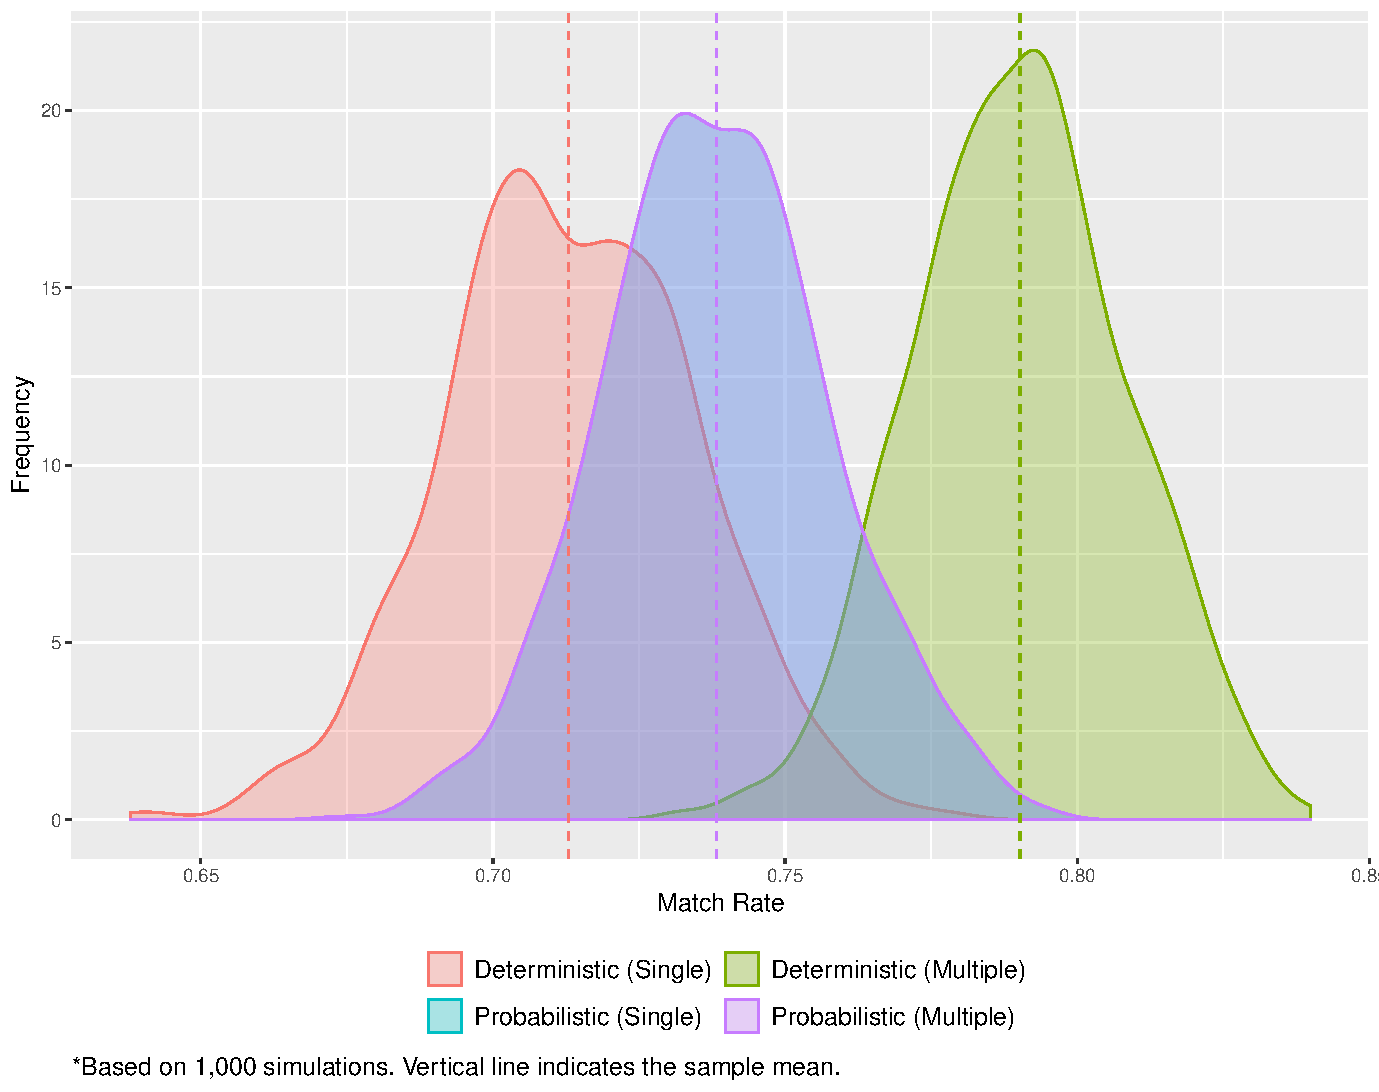
\includegraphics[width=\textwidth]{./Figures/match_rate.pdf}
\label{match_hist}
\end{center}
\end{figure}



I compare also ABE Multi and PRL Multi to determine whether the probability of containing a true match increases by allowing for multiple matches (Table \ref{multi_tab}).   In both procedures, more than half of observations are matched to a unique outcome, and those outcomes are correct 99 and 97 percent of the time for ABE Multi and PRL Multi, respectively.   Essentially, allowing for multiple matches in the deterministic procedure increases the probability that the true match is contained among the possible matches.  

\subsection{Estimation Results}

\section{Discussion}
To what extent my results generalize beyond the simulated data is unclear.  Many arbitrary choices -- name dictionary choice, uniform probability over those names -- and how I introduced error in the identifying variables may impact my results in important ways.  This needs to be studied in more detail, ideally with real data where a ground truth is also available. 

%  Multi Match Table 




I evaluate the performance of the matching procedures and estimation procedures using the following criteria.  For the matching procedures, I calculate

I compare estimators according to median absolute deviation.  I plot a histogram of the estimators. 


\section{Implementation Notes}
Here I will talk about all the nit-picky stuff, like 
\begin{itemize}
\item what threshold level I use for the fastLink algorithm (0.6)
\item what nonparametric technique I use for AHL (nearest neighbor) 
\item how I choose z in LL when there are multiple matches (randomly)
\item how I calculate standard errors for all of the estimators (using formulas for now)
\item how I standardize the variables for matching (nysiis function in R)
\item I change Step 2 in the ABE algorithm to restrict the all observations with unique first name, last name, date of birth, and $(x_1, x_2)$ combinations. 
\item  When allowing for multiple matches, I count as matches all record pairs with the same name, and the difference in recorded birth years is within two (or five) years.  That is, I designate all potential matches that arise in Step 3 as matches. 
\end{itemize}

\section{Results}
In total, I will test three DGPs (two now; more in Monte Carlo). The first is exactly as described in Section 2.  The second allows for correlation  between $x_1$ and the probability of an error.  The third will allow for correlation between $y$ and the probability of an error. 

The $y$ are generated according to the same DGP described above; that is the true $\beta_0 = (2, 0.5, 1)$.  I compare my results to an oracle linkage method (``first best"), which would successfully link all 400 $x$ observations to their correct $y$.  

I haven't finished coding, but here is an overview of the figures and tables so far:
\begin{itemize}
\item Table \ref{match_rate} shows the number of matches, percent correct, and number of uniquely matched $x_i$ for each matching method.  We see that no method is able to match every observation in the $x$ datafile.  The ABE method performs the best, but I also use a small threshold for PRL that could potentially be adjusted in order to achieve similar performance. 
\item Table \ref{naive} shows the OLS results applied naively (without any corrections for double counting $x$ with multiple $y$) to each of the matched datasets.  The First Best estimator is the benchmark case, produced by perfectly matched data. 
\item Another way to view the output of the matching algorithms is Figure \ref{match_plot} (but this is kind of messy and maybe a QQ plot is better?)
\item Figure \ref{nMatches} shows the distribution of $L_i$ for methods that create multiple matches.  
\item Table \ref{estimates} contains parameter estimates and standard errors (not always correcT) for different estimation methods on different datasets that can be compared to the naive OLS.
\end{itemize}% results here


% Naive OLS Table
\begin{table}[h!]
\let\center\empty
\let\endcenter\relax
\centering
\caption{Naive OLS for all of the matchings}
\resizebox{\textwidth}{!}{
% Table created by stargazer v.5.2.2 by Marek Hlavac, Harvard University. E-mail: hlavac at fas.harvard.edu
% Date and time: Wed, Oct 02, 2019 - 11:22:55
\begin{tabular}{@{\extracolsep{5pt}}lccccc} 
\\[-1.8ex]\hline 
\hline \\[-1.8ex] 
 & \multicolumn{5}{c}{\textit{Dependent variable:}} \\ 
\cline{2-6} 
\\[-1.8ex] & \multicolumn{5}{c}{y} \\ 
 & First Best & ABE (Single) & ABE (Multi) & PRL (Single) & PRL (Multi) \\ 
\hline \\[-1.8ex] 
 x1 & 0.408$^{***}$ & 0.413$^{**}$ & 0.369$^{**}$ & 0.587$^{***}$ & 0.357$^{**}$ \\ 
  & (0.143) & (0.172) & (0.153) & (0.180) & (0.168) \\ 
  & & & & & \\ 
 x2 & 1.096$^{***}$ & 1.010$^{***}$ & 0.905$^{***}$ & 0.975$^{***}$ & 0.930$^{***}$ \\ 
  & (0.052) & (0.062) & (0.056) & (0.065) & (0.062) \\ 
  & & & & & \\ 
 Constant & 2.079$^{***}$ & 2.106$^{***}$ & 2.100$^{***}$ & 1.932$^{***}$ & 2.091$^{***}$ \\ 
  & (0.102) & (0.125) & (0.109) & (0.131) & (0.122) \\ 
  & & & & & \\ 
\hline \\[-1.8ex] 
Observations & 400 & 327 & 454 & 311 & 373 \\ 
R$^{2}$ & 0.534 & 0.455 & 0.367 & 0.429 & 0.384 \\ 
Adjusted R$^{2}$ & 0.532 & 0.452 & 0.364 & 0.425 & 0.381 \\ 
\hline 
\hline \\[-1.8ex] 
\textit{Note:}  & \multicolumn{5}{r}{$^{*}$p$<$0.1; $^{**}$p$<$0.05; $^{***}$p$<$0.01} \\ 
\end{tabular} 
}
\label{naive}
\end{table}

% match plot
\begin{figure}[htbp]
\label{match_plot}
\caption{$(x,y)$ pairs produced by different matching algorithms}
\begin{center}
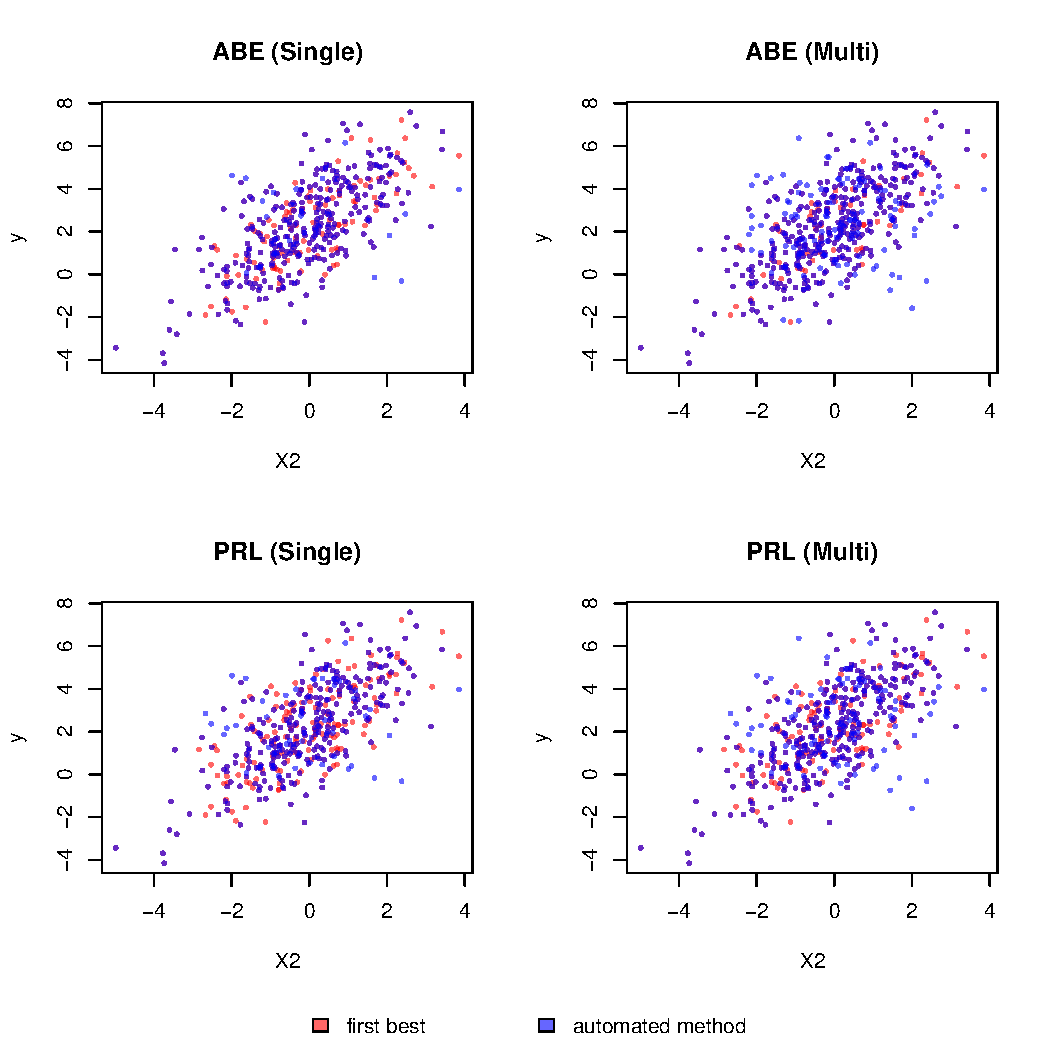
\includegraphics[width=\textwidth]{./Figures/match_plots.pdf}
\label{default}
\end{center}
\end{figure}

\begin{table}[htdp]
\label{estimates}
\let\center\empty
\let\endcenter\relax
\centering
\caption{Parameter estimates for different matched datasets and estimation procedures}
\vspace{10pt}
 \addtolength{\leftskip} {-1.5cm} 
 \addtolength{\rightskip}{-1cm}
\resizebox{1.2\textwidth}{!}{% latex table generated in R 3.5.1 by xtable 1.8-3 package
% Mon Oct  7 19:01:11 2019
\begin{tabular}{lrrrrrrrrrrrr}
  \hline
  & \multicolumn{4}{c}{AHL} & \multicolumn{4}{c}{SW} & \multicolumn{4}{c}{LL} \\

                             \cmidrule(lr){2-5}\cmidrule(lr){6-9}\cmidrule(lr){10-13} Parameter& ABE-M & ABE-S & PRL-M & PRL-S& ABE-M & ABE-S & PRL-M & PRL-S& ABE-M & ABE-S & PRL-M & PRL-S\\
 \hline
\$$\backslash$beta\_1\$ & 2.07 & 2.13 & 2.09 & 2.13 & 2.75 & 2.13 & 2.53 & 2.13 & 2.00 & 2.13 & 2.08 & 2.13 \\ 
   & 0.13 & 0.13 & 0.14 & 0.13 & 0.02 & 0.02 & 0.02 & 0.02 & 0.00 & 0.00 & 0.00 & 0.00 \\ 
  \$$\backslash$beta\_2\$ & 0.53 & 0.40 & 0.46 & 0.37 & 0.29 & 0.40 & 0.38 & 0.37 & 0.48 & 0.40 & 0.40 & 0.37 \\ 
   & 0.17 & 0.18 & 0.19 & 0.18 & 0.04 & 0.03 & 0.05 & 0.03 & 0.00 & 0.00 & 0.00 & 0.00 \\ 
  \$$\backslash$beta\_3 & 1.07 & 1.00 & 1.06 & 0.97 & 1.07 & 1.00 & 1.08 & 0.97 & 0.97 & 1.00 & 1.00 & 0.96 \\ 
   & 0.06 & 0.06 & 0.07 & 0.06 & 0.01 & 0.00 & 0.01 & 0.00 & 0.00 & 0.00 & 0.00 & 0.00 \\ 
   \hline
\end{tabular}
}
\end{table}


\section{Conclusion}
Will write when I have results. 





\newpage
\singlespacing
\bibliography{./Deadlines/proposal_bib} 
\bibliographystyle{aer}

\end{document}